\documentclass[pdf,aspectratio=169,10pt]{beamer}
\usetheme{%
%Berlin%
%Antibes%
%Boadilla%
%Copenhagen%
%Darmstadt%
%Frankfurt%
%Ilmenau%
%JuanLesPins%
%Madrid%
%Warsaw%
%Marburg%
%Boadilla%
simple%
}


%\usepackage{pgfpages}
%\pgfpagesuselayout{4 on 1}[a4paper,border shrink=5mm]
%\usepackage{scalefnt}
%\usepackage[version=4]{mhchem}
%\newcommand{\bftab}{\fontseries{b}\selectfont}
\usepackage{multirow}
\newcommand{\rot}[1]{\multirow{9}{*}{\rotatebox[origin=c]{90}{#1}}}
%\mode<presentation>


%\usecolortheme[RGB={15,90,0}]{structure}
%\usecolortheme[RGB={20,100,0}]{structure}
%\usecolortheme[RGB={10,80,0}]{structure}

\useinnertheme{circles}
%\useoutertheme{miniframes}
%\useoutertheme{shadow}
%\useoutertheme[subsection=false]{smoothbars}
%\useoutertheme{infolines}

% \usepackage[brazil]{babel}
%\usepackage[T1]{fontenc}
%\usepackage{ae} 
\usepackage[utf8]{inputenc} 
\usepackage[T1]{fontenc}


\usepackage{media9}      

\usepackage[onecol]{hackthefootline}
%\htfconfig{title=short, framenrs=counter, atsep=space}
\usepackage{algorithm}
\usepackage{algorithmic}
\usepackage{graphics}
\usepackage{graphicx}
%\usepackage[caption=false]{subfig}
\usepackage{caption}
%\usepackage{subcaption}
\usepackage{array} %for vertical thick lines in tables
\usepackage{multirow} %multirow tables
\usepackage{nicefrac} %for fractions like 1/4
\usepackage{booktabs}
\usepackage{multicol}
\usepackage{amssymb}
\usepackage{amsmath} 
\usepackage[makeroom]{cancel}
\usepackage{bm}
\usepackage[group-separator={,},separate-uncertainty]{siunitx}
\usepackage[most]{tcolorbox}
\usepackage{xcolor}
\usepackage[export]{adjustbox}

%\usefonttheme[onlymath]{serif}
%\usepackage{lmodern}
\usepackage{makecell}
%% Commande TikZ
\usepackage{tikz}
\usepackage{tikz,pgf,tikz-3dplot}
\usepackage{pgfplots}
\pgfplotsset{compat=1.16}
\usepackage[beamer]{hf-tikz}
\usetikzlibrary{bayesnet,shapes,arrows,positioning}
\tikzstyle{arrow} = [thick,->,>=stealth]
\tikzset{
	%Define standard arrow tip
	>=stealth',
	%Define style for boxes
	punkt/.style={
		rectangle,
		rounded corners,
		draw=black, very thick,
		text width=6.5em,
		minimum height=2em,
		text centered},
	% Define arrow style
	pil/.style={
		->,
		thick,
		shorten <=2pt,
		shorten >=2pt,}
}


\tikzstyle{rempliRed}=[red!30, fill=red!30]
\tikzstyle{ecritRed}=[red!60, fill=red!60]
\tikzstyle{rempliBlue}=[blue!30, fill=blue!30]
\tikzstyle{ecritBlue}=[blue!60, fill=blue!60]

\definecolor{color1}{rgb}{0.25, 0, 0.75}
\definecolor{color2}{rgb}{0.5, 0, 0.5}
\definecolor{color3}{rgb}{0.75, 0, 0.25}

\pgfplotsset{
    dirac/.style={
        mark=triangle*,
        mark options={scale=2},
        ycomb,
        scatter,
        visualization depends on={y/abs(y)-1 \as \sign},
        scatter/@pre marker code/.code={\scope[rotate=90*\sign,yshift=-2pt]}
    }
}

\def\mathunderline#1#2{\color{#1}\underline{{\color{black}#2}}\color{black}}

\DeclareMathOperator{\Tr}{\mathrm{Tr}}
\DeclareMathOperator{\KL}{\mathrm{KL}}
\usepackage{dsfont}


\newcommand{\E}[2][]{
   \ifthenelse{ \equal{#1}{} }
      {\ensuremath{\left\langle#2\right\rangle}}
      {\ensuremath{\left\langle#2\right\rangle_{#1}}}
}

\newcommand{\cov}[2][]{
    \ifthenelse{ \equal{#1}{} }
        {\operatorname{cov}\parens*{#2}}
        {\operatorname{cov}_{#1}\parens*{#2}}
}

%Felipe's packages


% Definitions
\newcommand*{\defeq}{\stackrel{\text{def}}{=}}
\newcommand{\tr}[1]{\operatorname{tr}\left(#1\right)}

\newcommand{\MOGP}{\ensuremath{\mathcal{MOGP}}}
\renewcommand{\L}{{\mathbb L}}
\def\data{\text{data}}
\def\sn{\sigma_{\text{noise}}}
\def\eye{\mathbf{I}}
\def\cN{{\mathcal{N}}}
\def\cX{{\mathcal{X}}}
\def\cY{{\mathcal{Y}}}
\def\dxi{{\text d} \xi}
\def\N{{\mathbb{N}}}
\def\m{{\mathbf{m}}}
\def\NLL{{\text{NLL}}}
\newcommand{\eps}{\varepsilon}
\def\R{{\mathbb{R}}}
\def\MVN{{\text{MVN}}}
\def\GP{{\mathcal {GP}}}
\def\y{{\mathbf{y}}}
\DeclareMathOperator{\OT}{OT}
\def\t{{\mathbf{t}}}
\def\x{{\mathbf{x}}}
\def\xizi{ \xi_0^{(i)} }
\def\u{{\mathbf{u}}}
\def\z{{\mathbf{z}}}
\def\X{{\mathbf{X}}}
\def\K{{\mathbf{K}}}
\def\dtau{{\text d\tau}}
\def\td{{\text d}}
\newcommand{\id}{\text{id}}



\newcommand{\fourier}[1]{\mathcal{F} \left\{#1\right\}}
\newcommand{\WF}[2]{\operatorname{WF}\left([#1],[#2]\right)}

\newcommand{\afourier}[1]{\mathcal{F}^{-1} \left\{#1\right\}}
\newcommand{\srp}[4]{\operatorname{simrect}_{#1,#2,#3}\left(#4\right)}
\newcommand{\rect}[1]{\text{rect}\left(#1\right)}
\def\sinc{ \operatorname{sinc} }
\newcommand{\SK}[1]{\operatorname{SK}\left(#1\right)}
\newcommand{\V}[2]{\mathbb{V}\left[#1,#2\right]}
\newcommand\eqdef{\overset{\mathrm{def}}{=}}
\newcommand{\GSK}[1]{\operatorname{GSK}\left(#1\right)}
\newcommand{\GSKN}[1]{\operatorname{GSK}_N\left(#1\right)}
\DeclareMathOperator\supp{supp}
\def\argmin{\mathop{\rm arg \; min}\limits}%
\def\diag{\mathop{\rm diag}\nolimits}%
%\let\leq=\leqslant
%\let\geq=\geqslant
%colours
\definecolor{navy}{HTML}{000080}
\providecommand{\rbullet}{{\textcolor{red}{{\bf \bullet}}}}
\providecommand{\bbullet}{{\textcolor{navy}{{\bf \bullet}}}}
\definecolor{clay}{RGB}{190,22,34}%
\providecommand{\bred}[1]{\textcolor{clay}{{\bf#1}}}
\providecommand{\bgreen}[1]{\textcolor{green}{{\bf#1}}}
\providecommand{\bteal}[1]{\textcolor{teal}{{\bf#1}}}
\providecommand{\bblue}[1]{\textcolor{navy}{{\bf#1}}}
\providecommand{\red}[1]{\textcolor{clay}{#1}}
\providecommand{\blue}[1]{\textcolor{navy}{#1}}
\providecommand{\bbullet}{{\textcolor{navy}{{\bf \bullet}}}}




%% Commande TikZ
\tikzstyle{rempliRed}=[red!30, fill=red!30]
\tikzstyle{ecritRed}=[red!60, fill=red!60]
\tikzstyle{rempliBlue}=[blue!30, fill=blue!30]
\tikzstyle{ecritBlue}=[blue!60, fill=blue!60]

\newcommand{\er}[1]{{\color{red!60} #1}}
\newcommand{\eb}[1]{{\color{blue!60} #1}}


% Commandes
\newcommand{\bigslant}[2]{{\raisebox{.2em}{$#1$}\left/\raisebox{-.2em}{$#2$}\right.}} 
\newcommand{\Z}{{\mathbb Z}}
\renewcommand{\P}{{\mathbb P}}
\newcommand{\G}{{\mathbb G}}
\renewcommand{\L}{{\mathbb L}}
\newcommand{\T}{{\mathbb T}}
\newcommand{\Q}{{\mathbb Q}}


\newcommand{\PP}{{\mathcal P}}
\newcommand{\HH}{{\mathcal H}}
\newcommand{\DD}{{\mathcal D}}
\newcommand{\BB}{{\mathcal B}}
\newcommand{\MM}{{\mathcal M}}
\newcommand{\XX}{{\mathcal X}}
\newcommand{\YY}{{\mathcal Y}}
\newcommand{\NN}{{\mathcal N}}
\newcommand{\LL}{{\mathcal L}}
\newcommand{\1}{{\mathds 1}}

\newcommand{\bX}{\boldsymbol{X}}
\newcommand{\bY}{\boldsymbol{Y}}
\newcommand{\bnu}{\boldsymbol{\nu}}
\newcommand{\bmu}{\boldsymbol{\mu}}
\newcommand{\boldeta}{\boldsymbol{\eta}}
\newcommand{\bsigma}{\boldsymbol{\sigma}}
\newcommand{\balpha}{\boldsymbol{\alpha}}
\newcommand{\bfun}{\boldsymbol{f}}
\newcommand{\bGamma}{\boldsymbol{\Gamma}}
\newcommand{\br}{\boldsymbol{r}}
\newcommand{\bq}{\boldsymbol{q}}
\newcommand{\bG}{\boldsymbol{G}}
\newcommand{\tH}{\tilde{H}}
\newcommand{\tg}{\tilde{g}}
\newcommand{\tS}{\tilde{\Sigma}}
\def\d{{\text d}}
\def\ba{ \boldsymbol{a} }
\def\bb{ \boldsymbol{b} }
\def\bx{ \boldsymbol{x} }
\def\by{ \boldsymbol{y} }




\newcommand{\CB}[1]{{\color{blue} #1}}
\newcommand{\CR}[1]{{\color{red} #1}}
\newcommand{\CV}[1]{{\color{green} #1}}
\newcommand{\CVI}[1]{{\color{violet} #1}}
\newcommand{\CP}[1]{{\color{purple} #1}}
\newcommand{\CO}[1]{{\color{orange} #1}}
\newcommand{\CM}[1]{{\color{magenta} #1}}
\newtheorem{proposition}{Proposition}  
\newtheorem{remark}{Remark}  



%imports
\usepackage[export]{adjustbox}
\usepackage[absolute,overlay]{textpos}
\setlength{\TPHorizModule}{\textwidth}
\setlength{\TPVertModule}{\textwidth}
\usepackage{soul}

% Pausing in the align environment
\makeatletter
\let\save@measuring@true\measuring@true
\def\measuring@true{%
  \save@measuring@true
  \def\beamer@sortzero##1{\beamer@ifnextcharospec{\beamer@sortzeroread{##1}}{}}%
  \def\beamer@sortzeroread##1<##2>{}%
  \def\beamer@finalnospec{}%
}
\makeatother

%listing package para código
\usepackage{listings}

\definecolor{codegreen}{rgb}{0,0.6,0}
\definecolor{codegray}{rgb}{0.5,0.5,0.5}
\definecolor{codepurple}{rgb}{0.58,0,0.82}
\definecolor{backcolour}{rgb}{0.95,0.95,0.92}
 
\lstdefinestyle{mystyle}{
	xleftmargin=0.05\textwidth,
	linewidth=0.95\textwidth,
    backgroundcolor=\color{backcolour},   
    commentstyle=\color{codegreen},
    keywordstyle=\color{magenta},
    numberstyle=\tiny\color{codegray},
    stringstyle=\color{codepurple},
    basicstyle=\ttfamily\scriptsize,
    breakatwhitespace=true,         
    breaklines=true,                 
    captionpos=b,                    
    keepspaces=true,                 
    numbers=left,                    
    numbersep=5pt,                  
    showspaces=false,                
    showstringspaces=false,
    showtabs=false,                  
    tabsize=2
}
 
\lstset{style=mystyle}
\usetikzlibrary{shapes.geometric,calc}

\newcommand\blobA[3][]%
{\draw[draw=black, fill=red!20] (#3) coordinate (#2-1)
     to [out=-90,in=-180] ++(0.5,-0.2) coordinate (#2-2)
     to [out=0,in=-180] ++(1.0,0.1) coordinate (#2-3)
     to [out=0,in=-180] ++(0.3,-0.1) coordinate (#2-4)
     to [out=0,in=-90] ++(0.2,0.2) coordinate (#2-5)
     to [out=90,in=-45] ++(-0.1,0.4)  coordinate (#2-6)
     to [out=135,in=-45] ++(-0.2,0.3)  coordinate (#2-7)
     to [out=135,in=0] ++(-0.2,0.2)  coordinate (#2-8)
     to [out=180,in=0] ++(-0.2,0.4)  coordinate (#2-9)
     to [out=180,in=45] ++(-0.2,-0.1)  coordinate (#2-10)
     to [out=-135,in=0] ++(-0.2,-0.1)  coordinate (#2-11)%	
     to [out=-180,in=45] ++(-0.3,-0.1)  coordinate (#2-12)
     to [out=-135,in=45]++(-0.3,0)  coordinate (#2-13)
     to [out=-135,in=90] (#2-1);
     \fill[draw=black, fill = red!30] (#2-1)	
   	to [out=-90,in=-180] ++(0.5,-0.2)
     to [out=0,in=-180] ++(1.0,0.1)
     to [out=0,in=-180] ++(0.3,-0.1)
     to [out=0,in=-90] ++(0.2,0.2) coordinate (#2-5);
  \fill[#1, color = red!30] (#2-5)
     to [out=90,in=0] ++(-1,0.3)  coordinate (#2-14)
     to [out=180,in=90] (#2-1);
   \draw[#1] (#2-5)
    to [out=90,in=0] ++(-1,0.3)  coordinate (#2-14)
    to [out=180,in=90] (#2-1);
	
	\draw[draw=black, fill=red!50] ++(1,0.1)  coordinate (#2-20)
    to [out=-90,in=180] ++(0.26,-0.13)  coordinate (#2-21)
    to [out=0,in=90]  (#2-20);  
    	\draw[draw=black, fill=red!50] ++(1,0.7)  coordinate (#2-22)
    to [out=-90,in=180] ++(0.26,0)  coordinate (#2-23)
    to [out=0,in=-90] ++(-0.1,0.2)  coordinate (#2-24)
     to [out=90,in=-45] ++(-0.1,0.1)  coordinate (#2-25)
	to [out=135,in=90]  (#2-22);
	\fill[color = red, opacity = 0.2] (#2-21)
	to [out=0,in=90]  (#2-20)
	to [out=90,in=90]  (#2-22)
	to [out=-90,in=180]	(#2-23)
	to [out=-90,in=90]  (#2-21);
  }
\newcommand\blobB[3][]%
  {\draw[draw=black, fill=blue!20]  (#3) coordinate (#2-1)
 	to [out=-90,in=-180] ++(0.4,-0.2) coordinate (#2-2)
     to [out=0,in=-180] ++(0.5,0.1) coordinate (#2-3)
     to [out=0,in=-180] ++(0.4,-0.1) coordinate (#2-4)
     to [out=0,in=-90] ++(0.8,0.1) coordinate (#2-5)
     to [out=90,in=-25] ++(-0.2,0.6)  coordinate (#2-8)
     to [out=155,in=20] ++(-0.2,0.2)  coordinate (#2-9)
     to [out=-160,in=0] ++(-0.2,0.3)  coordinate (#2-11)
     to [out=-180,in=30] ++(-0.5,-0.1)  coordinate (#2-12)
     to [out=-150,in=0] ++(-0.3,0.2)  coordinate (#2-12)
     to [out=-180,in=90] (#2-1);
   \fill[draw = black, fill = blue!30] (#2-1)
	to [out=-90,in=-180] ++(0.4,-0.2) coordinate (#2-2)
     to [out=0,in=-180] ++(0.5,0.1) coordinate (#2-3)
     to [out=0,in=-180] ++(0.4,-0.1) coordinate (#2-4)
     to [out=0,in=-90] ++(0.8,0.1) coordinate (#2-5);
     \fill[color = blue!30] (#2-5)
     to [out=90,in=0] ++(-0.2,0.1)  coordinate (#2-14)
     to [out=-180,in=15] ++(-1.2,0.2)  coordinate (#2-15)
     to [out=-165,in=25] ++(-0.2,0.1)  coordinate (#2-15)
     to [out=-155,in=90] (#2-1);
    \draw[#1] (#2-5)
     to [out=90,in=0] ++(-0.2,0.1)  coordinate (#2-14)
     to [out=-180,in=15] ++(-1.2,0.2)  coordinate (#2-15)
     to [out=-165,in=25] ++(-0.2,0.1)  coordinate (#2-15)
     to [out=-155,in=90] (#2-1);
     
    \draw[draw=black, fill=blue!50]  (#3)++(0.4,-0.1)  coordinate (#2-20)
	to [out=0,in=-90] ++(0.35,+0.2) coordinate (#2-21)
	to [out=90,in=135]  (#2-20);
	\draw[draw=black, fill=blue!50]  (#3)++(0.4,0.7)  coordinate (#2-22)
	to [out=-90,in=-135] ++(0.15,+0.02) coordinate (#2-23)
	to [out=45,in=-90] ++(0.2,+0.15) coordinate (#2-24)	
	to [out=90,in=35] ++(-0.2,-0.02) coordinate (#2-25)	
	to [out=-145,in=90]  (#2-22);
	\fill[color = blue, opacity = 0.2] (#2-21)
	to [out=90,in=135]  (#2-20)
	to [out=90,in=-90]  (#2-22)
	to [out=-90,in=-135] (#2-23)
	to [out=45,in=-90] (#2-24)
	to [out=-90,in=90]	(#2-21);
  }
  


\beamertemplatenavigationsymbolsempty
\setbeamertemplate{caption}[numbered]

\title[Tobar, A hands-on tutorial on Optimal Transport]{A hands-on tutorial on Optimal Transport
}
\author[]{Felipe Tobar}
\institute[]{Department of Mathematics \& I-X\\ Imperial College London}

\date{22 May, 2025}  


\begin{document}

\begin{frame}[plain]
    \titlepage
    \footnotesize
    \flushright{
    \bblue{ 
    \href{https://github.com/felipe-tobar/OT-tutorial/}{\texttt{github.com/felipe-tobar/OT-tutorial}}
    }
    }

    \begin{textblock}{0.45}(0.65,0.2)
        \begin{figure}
            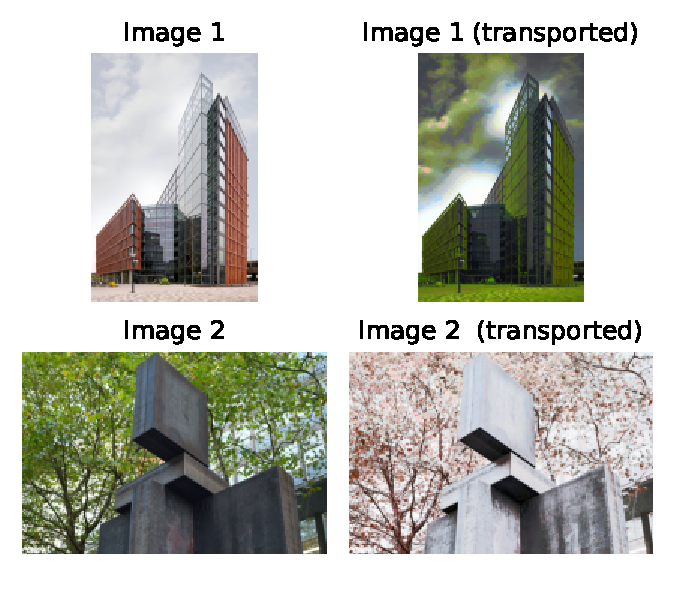
\includegraphics[trim={7cm 5cm 1cm 1cm},clip, height=0.45\textwidth]{../img/ex1_result.pdf}
        \end{figure}
    \end{textblock}

    \begin{textblock}{0.45}(-0.05,0.2)
        \begin{figure}
            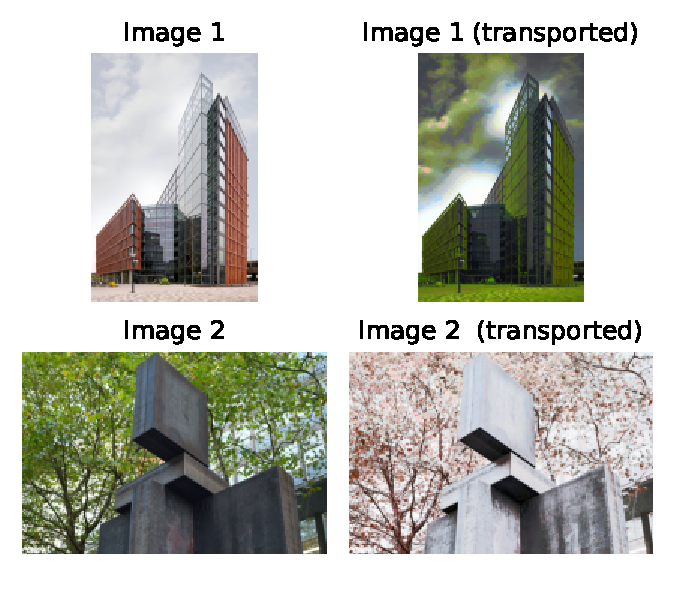
\includegraphics[trim={1cm 5cm 6.5cm 1cm},clip, height=0.45\textwidth]{../img/ex1_result.pdf}
        \end{figure}
    \end{textblock}



\end{frame}


\begin{frame}
    \frametitle{Overview} 
    \tableofcontents
\end{frame}


\section{Introduction}
\begin{frame}
\bred{Preliminary remarks}
\begin{itemize}
    \item Based on the Tutorial \bblue{Optimal Transport for Signal Processing} given at IEEE MLSP 2024 w/ Laetitia Chapel
    \item Examples based on \bblue{POT: Python Optimal Transport Toolbox} (\href{https://pythonot.github.io/}{\texttt{pythonot.github.io}})
    \item Tutorial repository: \bblue{ 
    \href{https://github.com/felipe-tobar/OT-tutorial/}{\texttt{github.com/felipe-tobar/OT-tutorial}}
    }
    \item To set up your environment (tested on OSX and Linux on 19 May 2025):
    \vspace{1em}
    \begin{tcolorbox}[colback=blue!5!white,colframe=blue!75!black]
    \centering
  \texttt{conda env create -f environment.yml}
\end{tcolorbox}


\end{itemize}
\vspace{3em}
\bblue{$\infty$ thanks to:} Elsa Cazelles (Toulouse), Fernando Fetis (U.~Chile), Marco Cuturi (Apple/ENSAE), Rémi Flamary (École Polytechnique) 

\end{frame}


\begin{frame}{
\bred{OT for data analysis in a nutshell}
}
\bblue{Optimal Transportation theory} is a set of tools for computing distances between distributions
\vspace{1em}

\begin{minipage}{0.5\textwidth}
\begin{figure}
  \includegraphics[width=0.99\textwidth]{../img/OT_shovel}
\end{figure}    
\end{minipage}
\hfill
\begin{minipage}{0.45\textwidth}
\bblue{We are interested in OT because}
\begin{itemize}
    \item it gives a geometric-based view of probability distributions 
    \item it enhances the machine learning (generative models), and data analysis (histograms) toolboxes.
    \item it addresses shortcomings of previous distances
    \item it is beautiful (but that's subjective)
\end{itemize}
\end{minipage}
\vfill

\tiny{Figure taken from \url{https://www.microsoft.com/en-us/research/blog/measuring-dataset-similarity-using-optimal-transport/}. \\Credit: David Alvarez-Melis \&  Nicolo Fusi (Microsoft Research)}

\end{frame}






\begin{frame}{Origins of OT: Old and New }
\bblue{Gaspard Monge (1781):} How to transport a pile of sand onto a hole in an optimal way?

  \begin{center}
  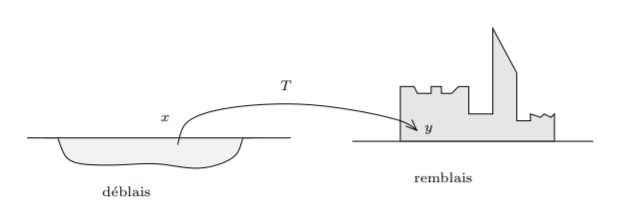
\includegraphics[height=2cm]{../img/deblais}\vspace{0.2cm}
  \end{center}

\bblue{Leonid Kantorovich (1942):} Generalisation of Monge's and dual formulation\\


\bblue{Yann Brenier (1987):} Connections w/ PDEs, fluid mechanics,
probability theory, and more. \\

\bblue{A number of Fields Medals (2010+)}  Villani, Hairer, Figalli\\

\bblue{Marco Cuturi (2013):} Breakthrough in Machine Learning

\end{frame}



\section{Part I\\ The Optimal Transport Problem}


\begin{frame}
    \Large \bblue{Part I\\ The Optimal Transport Problem}
\end{frame}



{
\usebackgroundtemplate{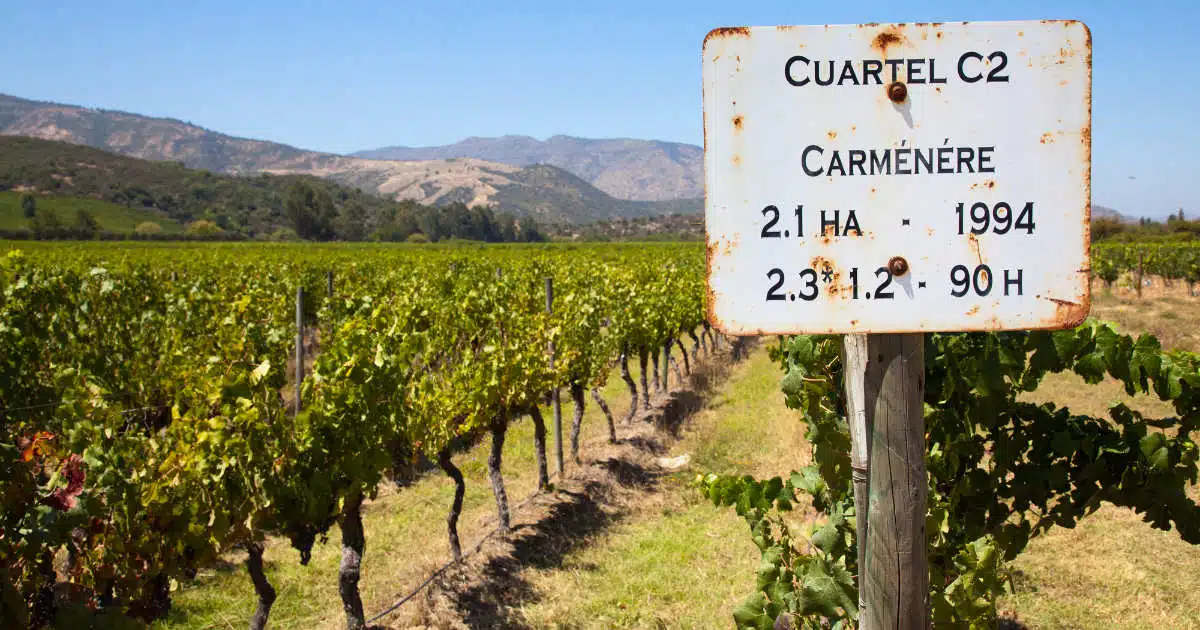
\includegraphics[width=\paperwidth]{../img/wine.png}}
\begin{frame}[plain]
\end{frame}
}



\begin{frame}{The assignment problem}
    \begin{figure}
        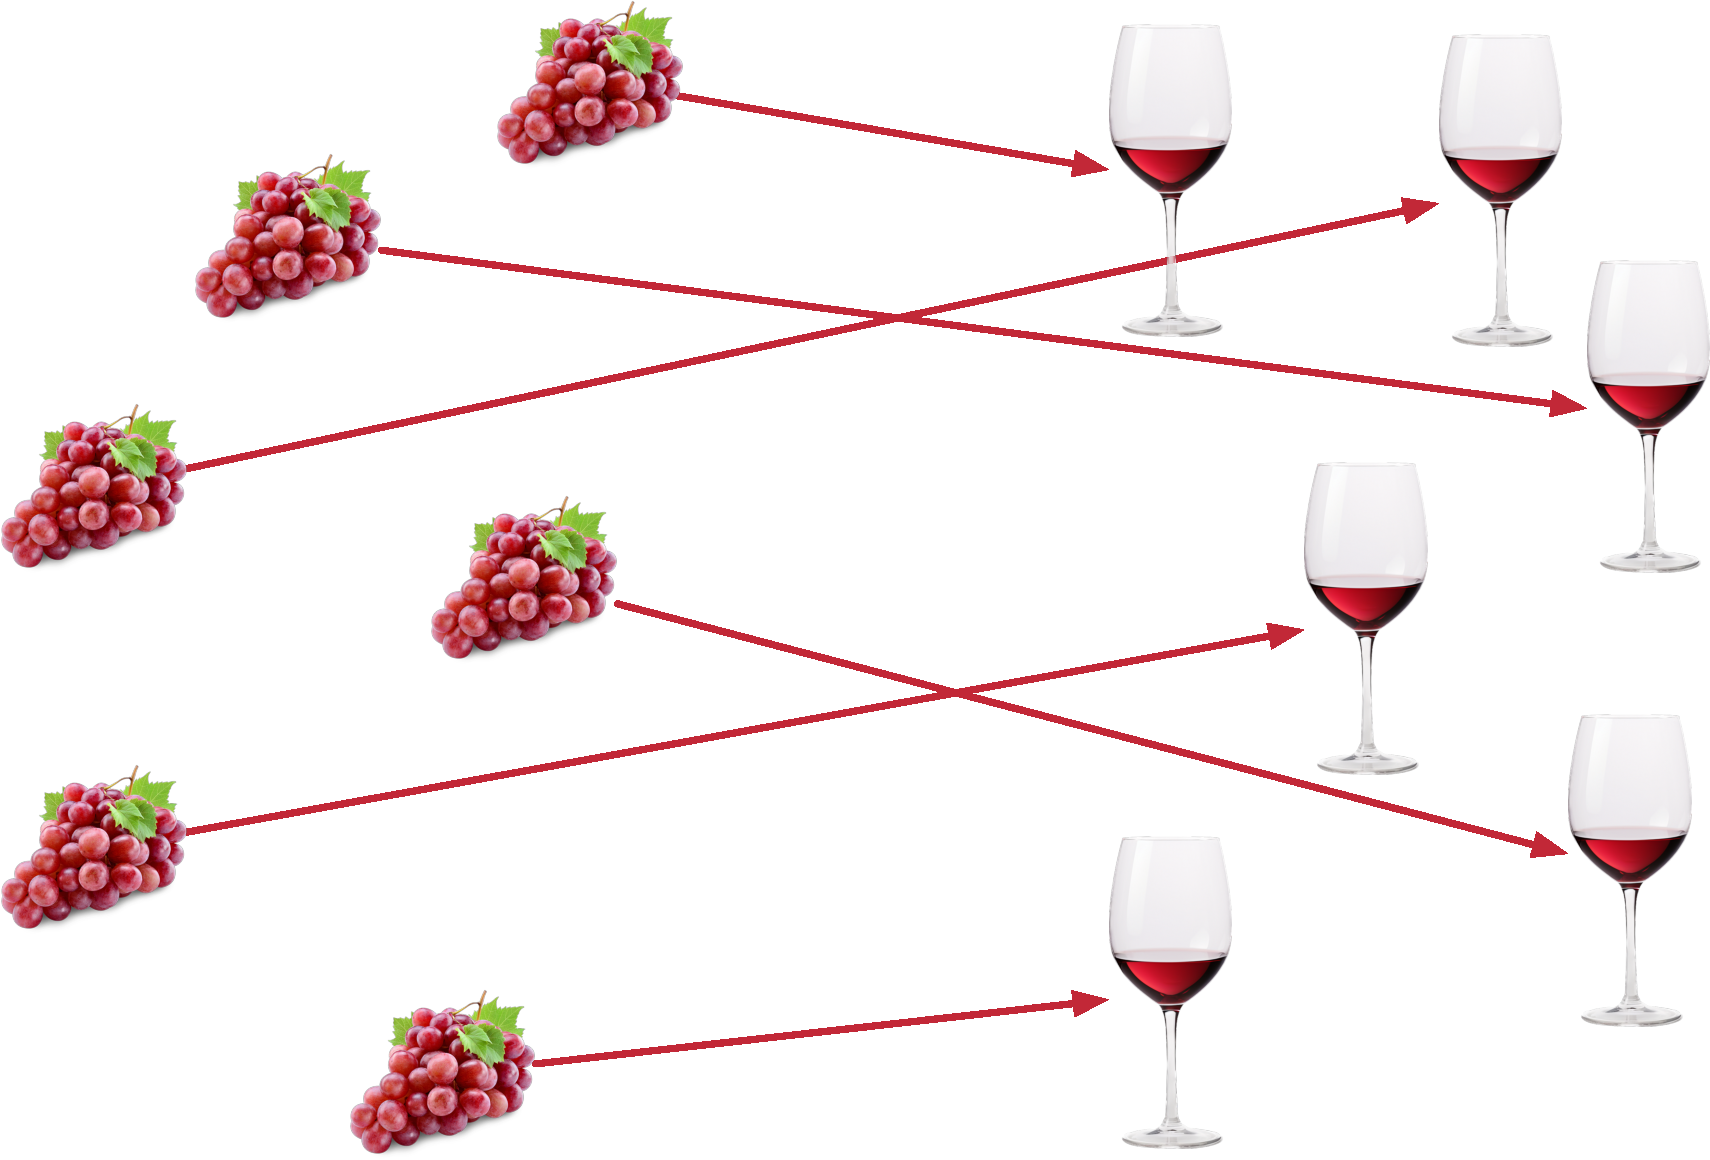
\includegraphics[height=0.7\textheight]{../img/wine_assignment.pdf}  
    \end{figure}
\end{frame}

\begin{frame}{The assignment problem: encoding the real world}

\begin{minipage}{0.45\textwidth}
\begin{itemize}
    \item Weighted masses
    \item Different number of sources/targets
    \item Straight path is not possible
    \item New source/target becomes available
\end{itemize}
\vspace{2em}
\centerline{ \bred{(we'll start with a simple case)} }
\end{minipage}
\hfill
\begin{minipage}{0.5\textwidth}
 \begin{figure}
        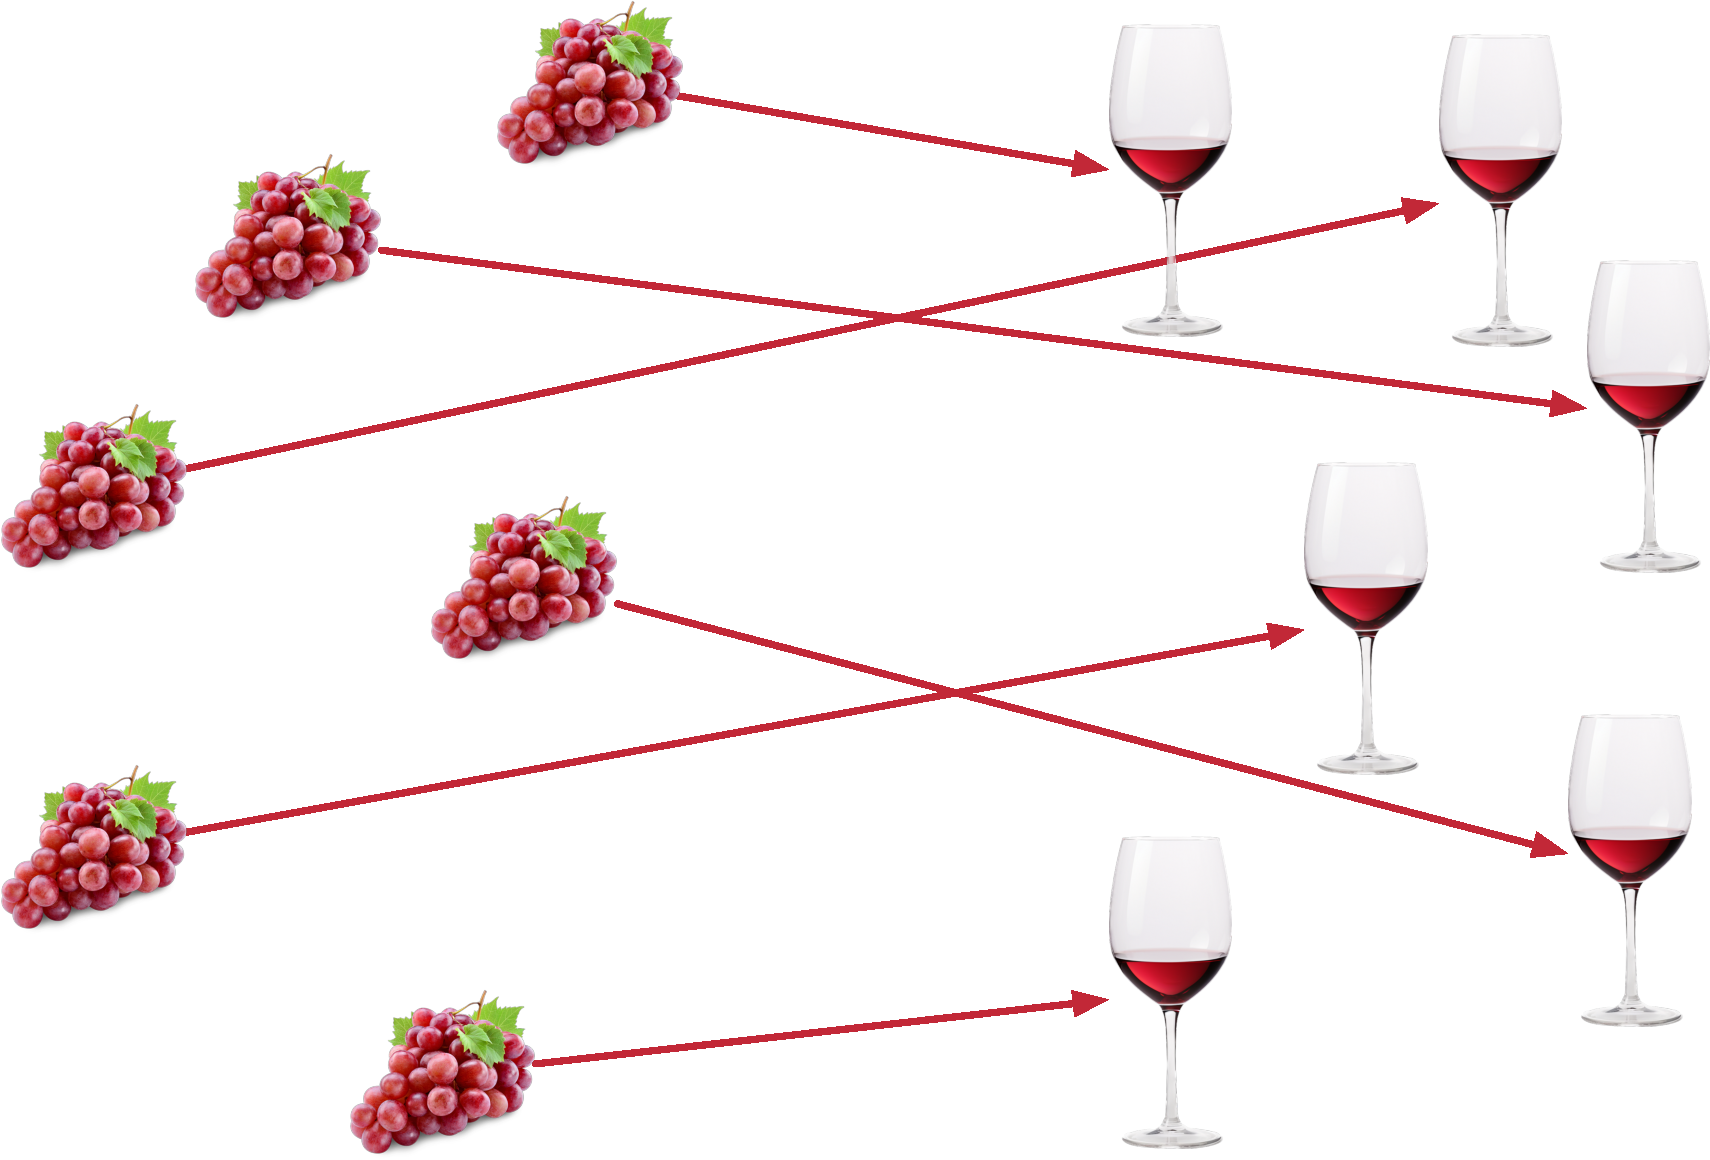
\includegraphics[width=0.99\textwidth]{../img/wine_assignment.pdf}  
    \end{figure}
\end{minipage}

\end{frame}


\begin{frame}[plain]{Monge formulation\footnote{Monge, G. (1781).
Mémoire sur la théorie des déblais et des remblais.
De l'Imprimerie Royale.}}
\bblue{Objective:} To move a pile of mass from one location to another at a minimum effort\\
\vspace{1em}

\begin{minipage}[t]{0.69\textwidth}
    \bred{Notation:} 
   \begin{itemize}
       \item \bblue{Piles of mass} are probability distributions, $\mu$ and $\nu$, corresponding to random variables $X\in\cX$ and $Y\in\cY$. 
       \item \bblue{Moving procedure} is a function $T: x \in \cX\mapsto y\in\cY$.
    \item \bblue{Moving cost} encoded as $c: (x,y)\in\cX\times\cY\mapsto c(x,y)\in\R$.
   \end{itemize}
\vspace{1em}

    \bred{Optimise} 
  the total transport cost
    \begin{equation}
        \OT{(\mu,\nu)} = \min_{T\in M_{X,Y}}\sum_{x\in\cX} c(x_i, T(x_i)),
    \end{equation}
     where $M_{X,Y} = \{ T: \cX \to \cY,\ s.t.,\ T_{\#\mu}=\nu \}$ is the space of \emph{admissible transport maps}.
\end{minipage}   
\hfill
\begin{minipage}[t]{0.3\textwidth}
\vspace{2em}
       \begin{tikzpicture}[>=stealth,scale=1.3]
\small
 \blobA[dashed]{a}{0,0}
  \blobB[dashed]{b}{1.5,-2}
   \node at(0.2,0) {$\XX$};
    \node at(3.2,-2.1) {$\YY$};
  \draw[->] (0.5,-0.4) to[bend right] node[above]{\hspace{1em}  $T$} (1.4,-2); 
  %\node at(1.5,-0.5) {\footnotesize $A=\{x\in\XX:T(x)\in B\}$};
% \node at(3.55,0) {\scriptsize $B$};
 %\draw[->] (0.75,-0.4) to (1.05,-0.05);   
 %\node at(6,0.5) {$T\#{\color{red!50} \mu} = {\color{blue!50} \nu}$};
  %\node at(6.3,0.2) {i.e., ${\color{red!50} \mu(A)} = {\color{blue!50} \nu(B)}$};
\end{tikzpicture}
\end{minipage}   

\end{frame}


\begin{frame}{The transport map (aka the \emph{pushforward} operator $T_\#$)}
    $T$ \emph{transports} mass from $\cX$ to $\cY$, meaning that for any subset $A\in\cY$, one has 
    \begin{equation}
        \nu(A) = \mu(T^{-1}(A)),
    \end{equation}
    where $T^{-1}(A)=\{x\in\cX, s.t.\ T(x)\in A \}$ is the preimage of $A$ under $T$.
\vspace{2em}

\begin{tikzpicture}[>=stealth,scale=1.75]
\small
 \blobA[dashed]{a}{0,0}
  \blobB[dashed]{b}{3,0}
   \node at(0.2,0) {$\XX$};
    \node at(3.2,0) {$\YY$};
  \draw[->] (1.8,1) to[bend left] node[above]{$T$} (3.1,1); 
  \node at(1.5,-0.5) {\footnotesize $A=\{x\in\XX:T(x)\in B\}$};
 \node at(3.55,0) {\scriptsize $B$};
 \draw[->] (0.75,-0.4) to (1.05,-0.05);   
 \node at(6,0.5) {$T\#{\color{red!50} \mu} = {\color{blue!50} \nu}$};
  \node at(6.3,0.2) {i.e., ${\color{red!50} \mu(A)} = {\color{blue!50} \nu(B)}$};
\end{tikzpicture}\\
\flushright{\small {(figure adapted from \href{https://www.damtp.cam.ac.uk/research/cia/files/teaching/Optimal_Transport_Notes.pdf}{Thorpe's book})}}
\end{frame}






\begin{frame}{\bred{Warning:} Neither existence nor uniqueness is guaranteed}
        \begin{figure}
        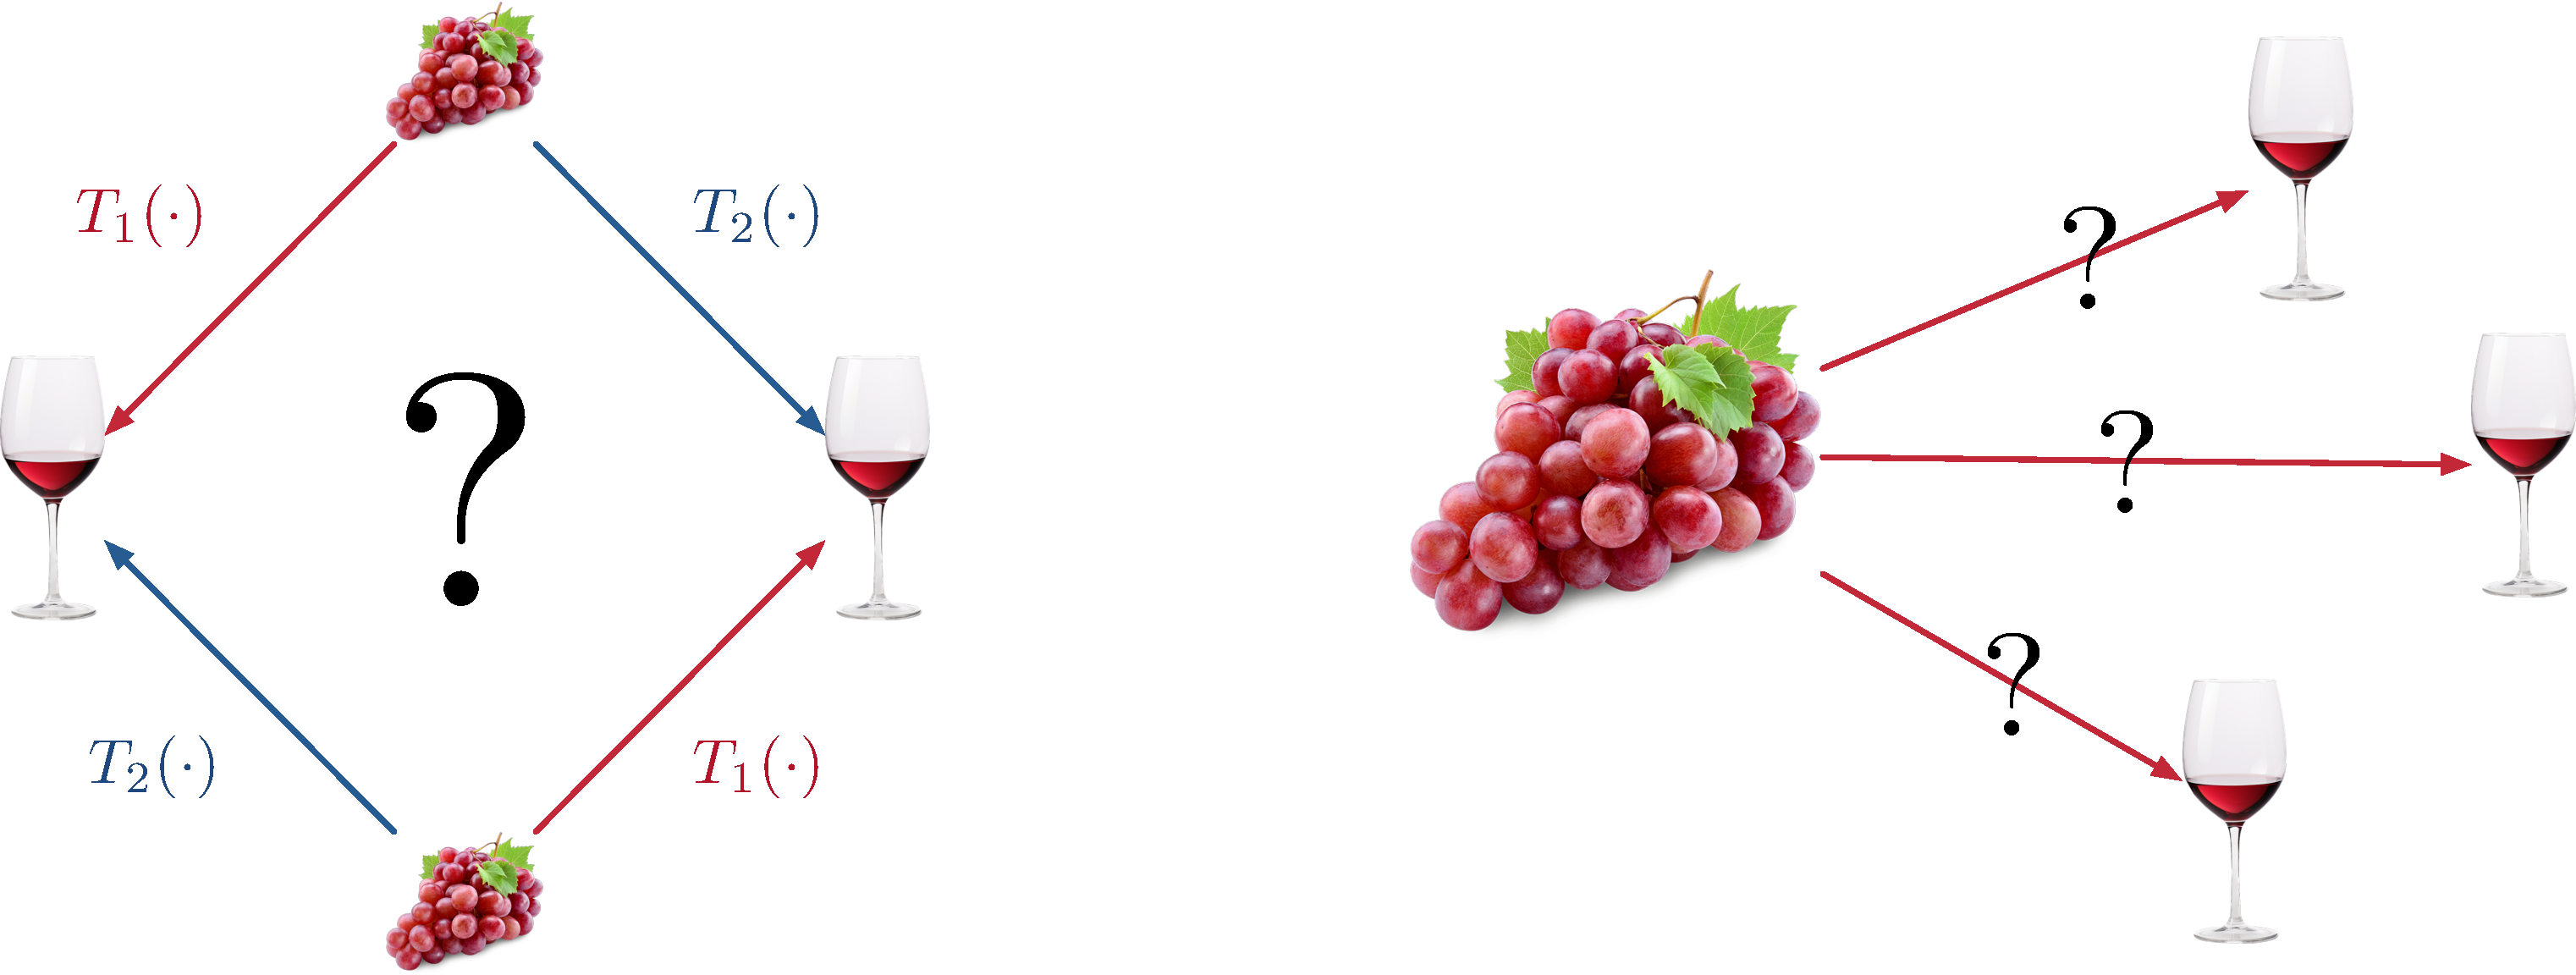
\includegraphics[width=0.7\textwidth]{../img/existence_uniqueness.pdf}
    \end{figure}
    \vspace{1em}
\bred{Remark:} When both distributions have the same number of same-weight atoms, e.g., pixels or class instances, Monge's formulation can be solved. However, when dealing with different number of \emph{weighted samples}, \textbf{Monge's map might be unable to transport the mass.}
\end{frame}


\begin{frame}{Kantorovich formulation: \onslide<3>{mass splitting}}

     \begin{figure}
        \includegraphics<1>[width=0.6\textwidth]{../img/wine_assignment.pdf}
        \includegraphics<3>[width=0.6\textwidth]{../img/wine_assignment_split.pdf}
        \includegraphics<2>[width=0.6\textwidth]{../img/wine_assignment_q.pdf}
    \end{figure}
\end{frame} 

\begin{frame}{Kantorovich's \emph{transport plan}} 
\begin{textblock}{0.35}(0.72,0.02)
     \begin{figure}
        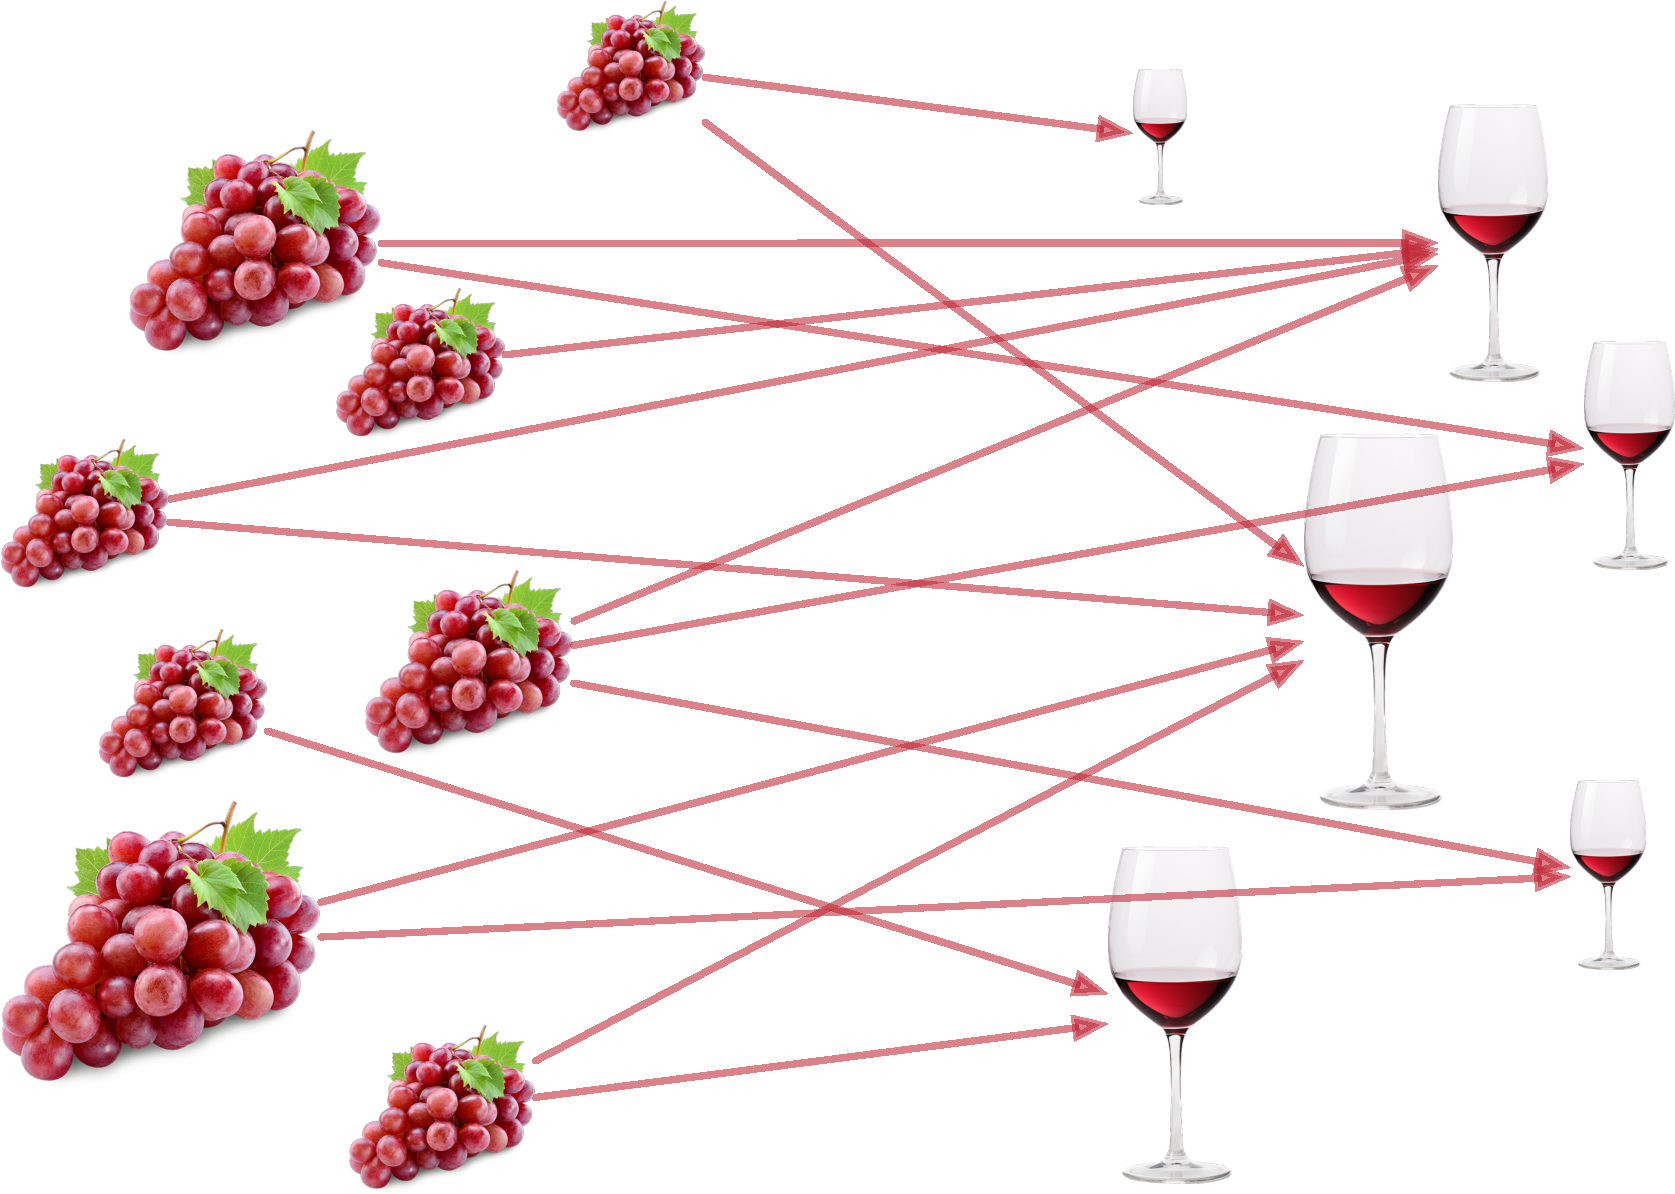
\includegraphics[width=0.6\textwidth]{../img/wine_assignment_split.pdf}
    \end{figure}
\end{textblock}

\begin{equation*}
    \hspace{-2em}\OT{(\mu,\nu)} = \inf_{P\in\Pi_{\mu,\nu}} \langle P , C\rangle = \sum_{i,j}^{n,m} C_{ij}P_{ij} 
\end{equation*}
where $\Pi_{\mu,\nu}  = \{  P\in {[0,1]}^{m\times n} :  \sum_{i=1}^m P_{ij} = \nu_j,  \sum_{j=1}^n P_{ij} = \mu_i \}$
    \begin{figure}
        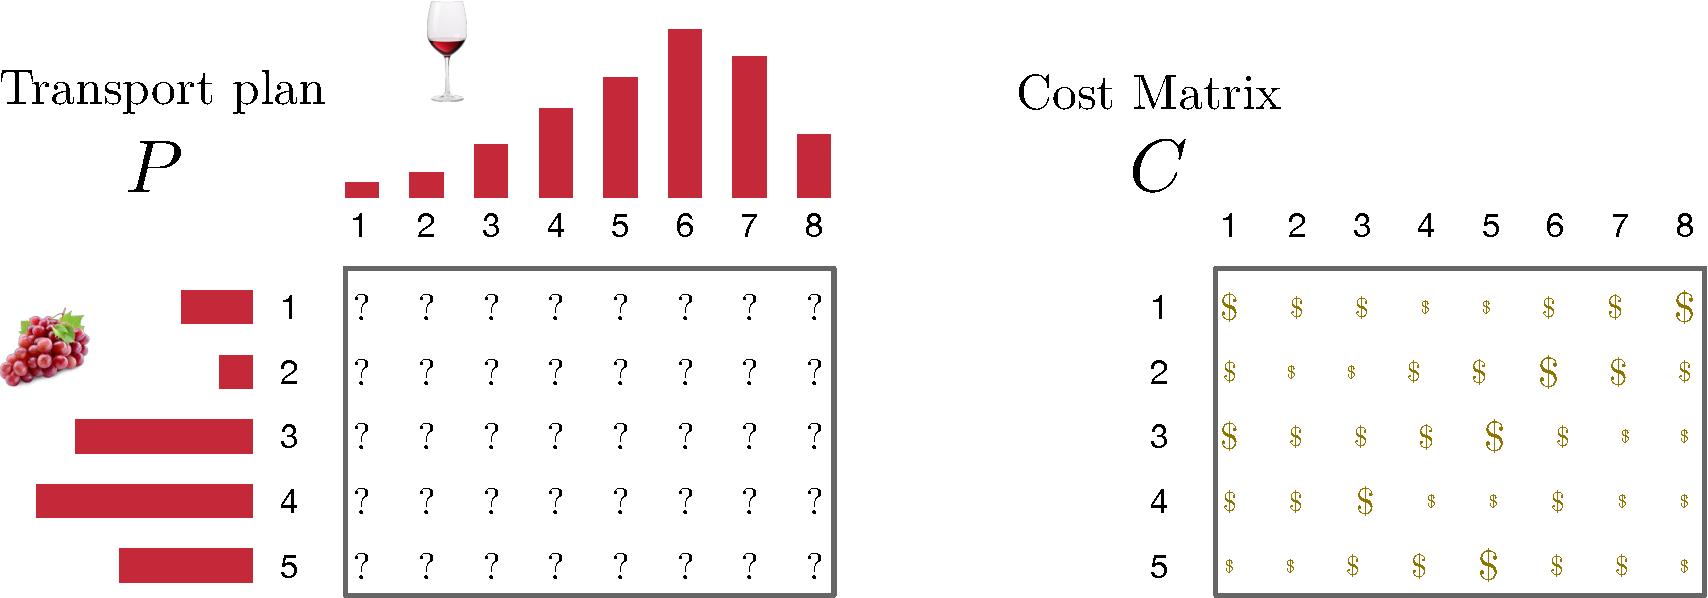
\includegraphics[width=0.9\textwidth]{../img/kantorovich.pdf}
    \end{figure}
\end{frame}

 

\begin{frame}{\bred{Example 0:} Compute transport plan (no toolbox)}
    Computing the OT requires solving a linear problem

\begin{minipage}{0.49\textwidth}  
\begin{equation*}
    \hspace{-2em}\OT{(\mu,\nu)} = \inf_{P\in\Pi_{\mu,\nu}}  \sum_{i,j}^{n,m} C_{ij}P_{ij} 
\end{equation*}
subject to
\begin{equation*}
    0\leq P_{ij} \leq 1, \sum_{i=1}^m P_{ij} = \nu_j,  \sum_{j=1}^n P_{ij} = \mu_i
\end{equation*}
Feasible set:
\begin{figure}
            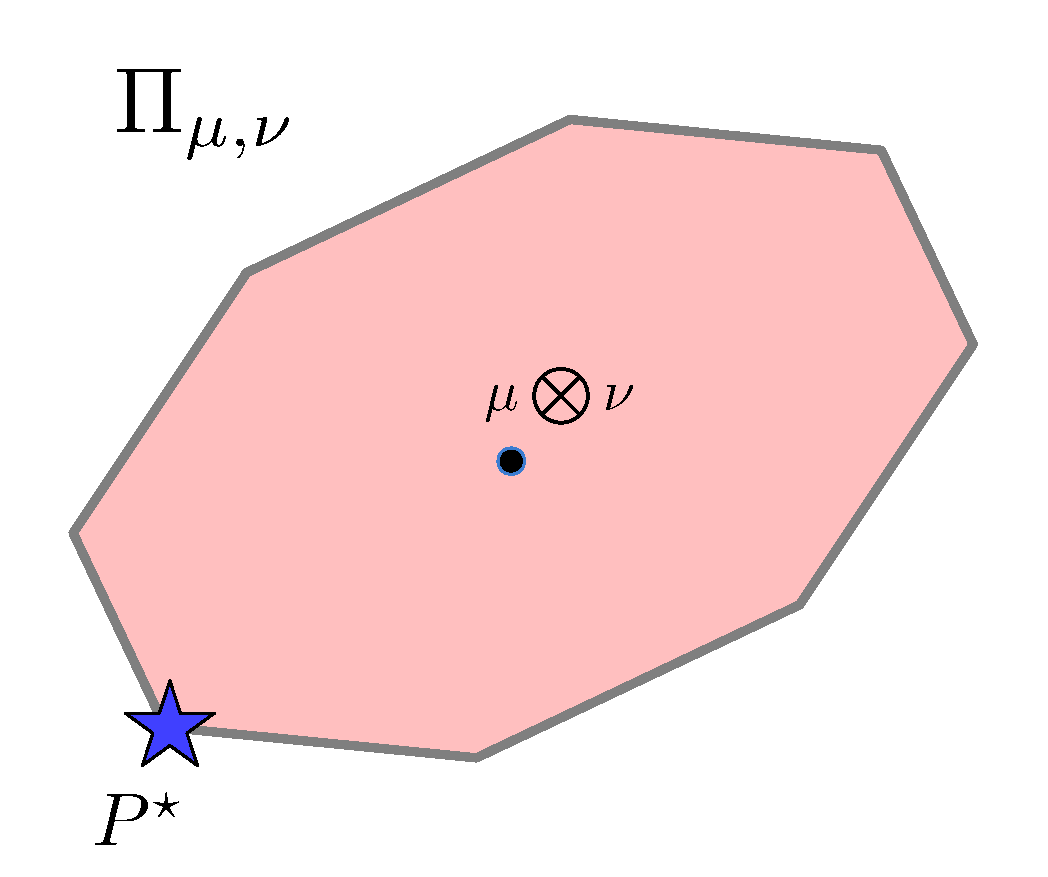
\includegraphics[width=0.48\textwidth]{../img/polytope1.pdf}\hspace{2em}

\end{figure}

\end{minipage}
\hfill
\begin{minipage}{0.49\textwidth}  
Algorithm:

\begin{itemize}
    \item Input: $\mu$ and $\nu$ with supports $s_\mu$ and $s_\nu$
    \item Check distributions are valid
    \item Compute $C = c(s_\mu,s_\nu)$
    \item Soln: $P^\star = \argmin \sum_{i,j}^{n,m} C_{ij}P_{ij} $
    \item Overall cost: $d = \sum_{i,j}^{n,m} C_{ij}P^\star_{ij}$ 
\end{itemize}
\end{minipage}

\begin{textblock}{0.45} (0.58,0.54)
\small
\bred{
\underline{
    Notebook: \href{https://github.com/felipe-tobar/OT-tutorial-MLSP-2024/blob/main/Codes/Wasserstein_linprog.ipynb}{Wasserstein\_linprog.ipynb}
}}
\end{textblock}
\end{frame}




\begin{frame}{\bred{Example 1:} Discrete Kantorovich plan}
    Let consider the following source and target distributions

\begin{minipage}{0.49\textwidth}  
\begin{figure}
        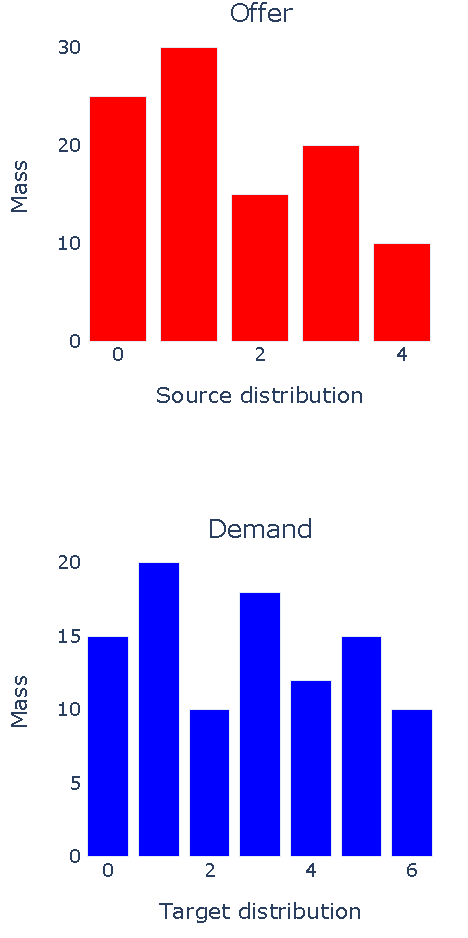
\includegraphics[width=0.48\textwidth]{../img/kantorovich_discrete_histogram.pdf}\hspace{2em}
    \end{figure}
\end{minipage}
\hfill
\begin{minipage}{0.49\textwidth}
\begin{figure}
        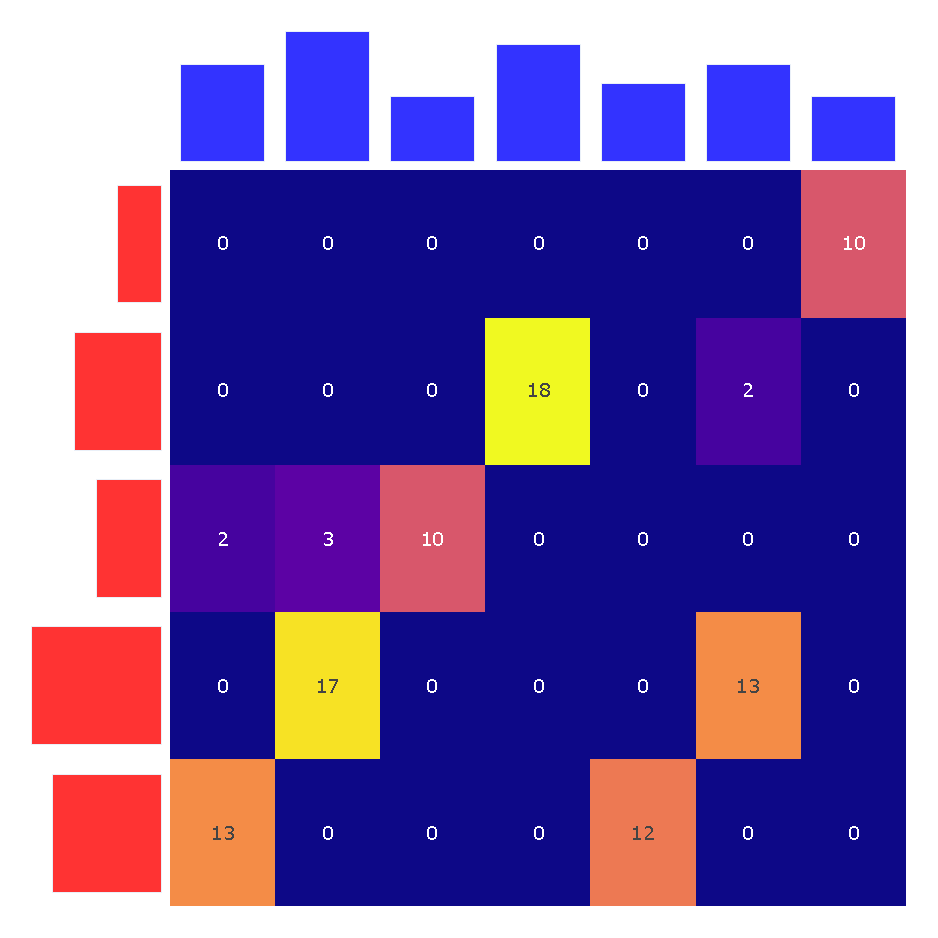
\includegraphics[width=0.8\textwidth]{../img/kantorovich_discrete_solution.pdf}\hspace{2em}
    \end{figure}
\end{minipage}

\begin{textblock}{0.45} (0.62,0.54)
\small
\bred{
\underline{
    Notebook: \href{https://github.com/felipe-tobar/OT-tutorial-MLSP-2024/blob/main/Codes/kantorovich.ipynb}{kantorovich.ipynb}
}}
\end{textblock}
\end{frame}






\begin{frame}{\bred{Example 2:} Continuous Kantorovich plan}
    Let us now consider two  distributions over a continuous support
\begin{minipage}{0.59\textwidth}
\begin{figure}
    \centering
        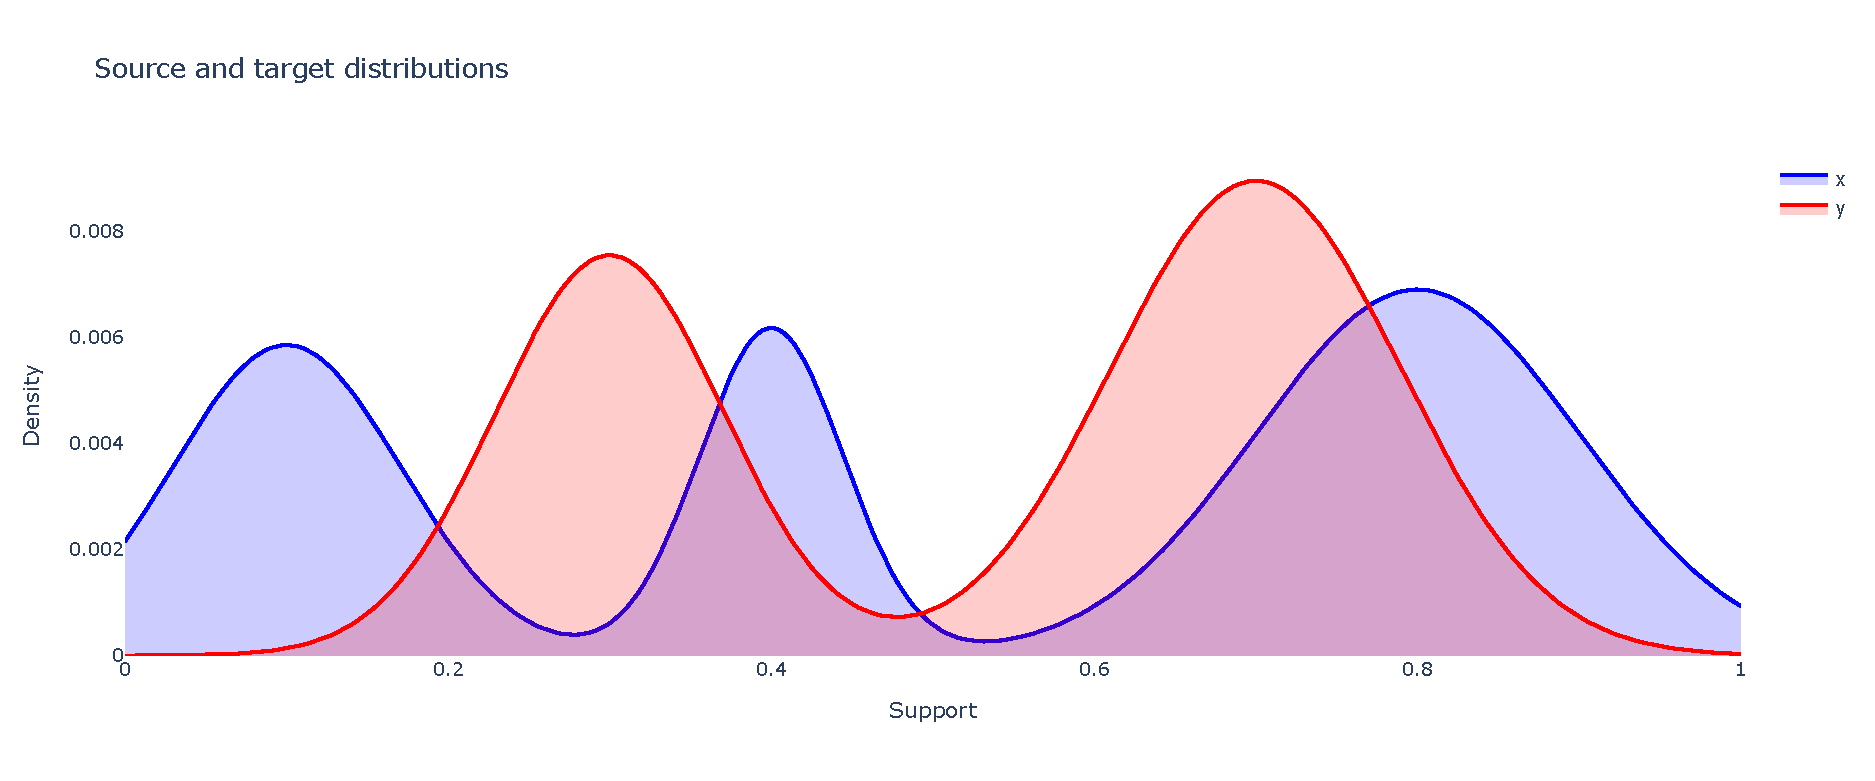
\includegraphics[width=0.9\textwidth]{../img/kantorovich_continuous_density.pdf}\hspace{2em}
    \end{figure}
            \bblue{Observe that the plan remained \emph{sparse}, i.e., the mass did not spread  much}

        (bear this in mind, explanation to follow)
\end{minipage} 
\hfill
\begin{minipage}{0.4\textwidth}
\begin{figure}
    \centering
        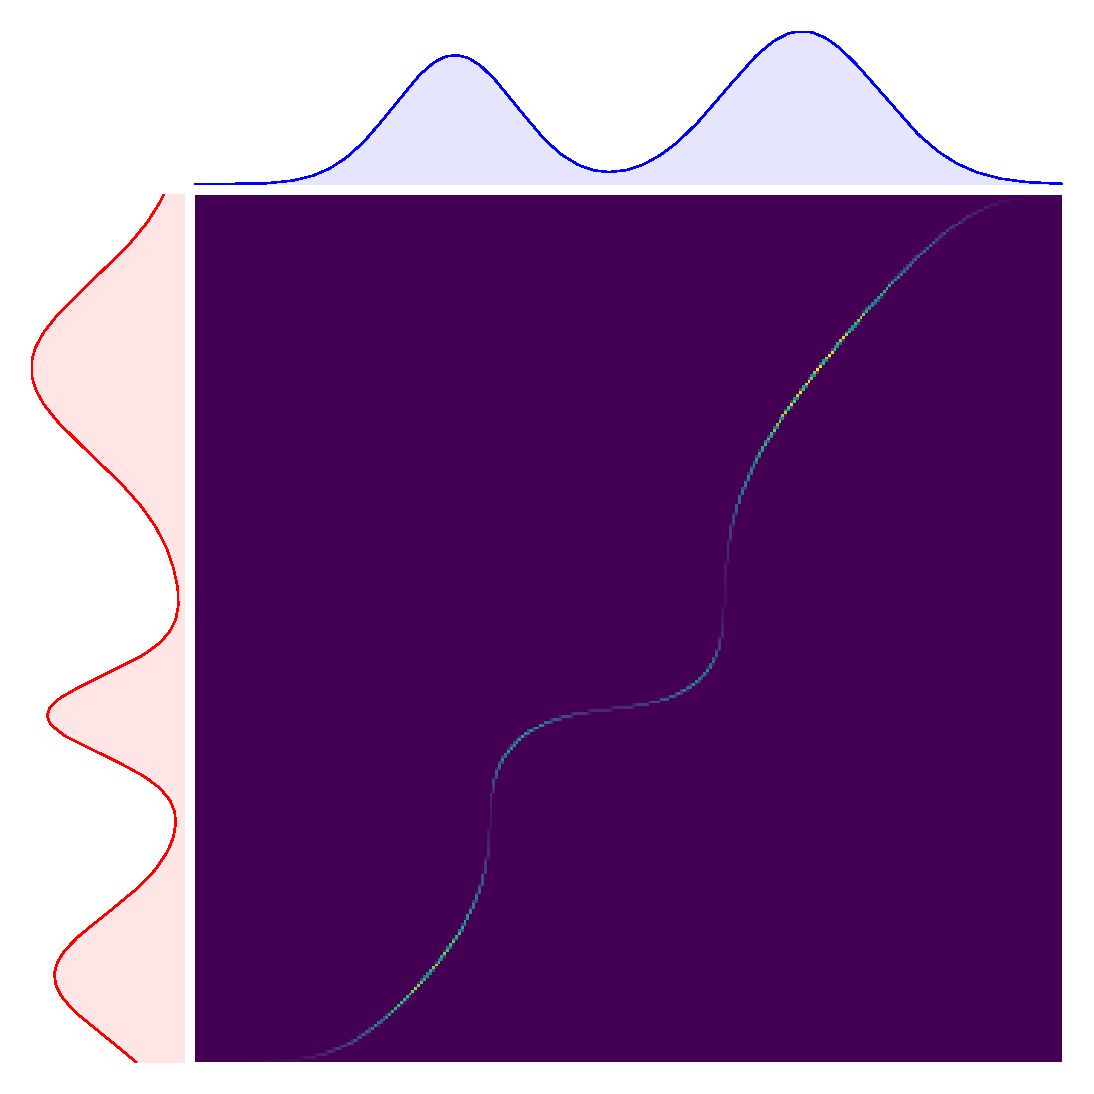
\includegraphics[width=0.9\textwidth]{../img/kantorovich_continuous_solution.pdf}
    \end{figure}
    \centering
    \small
\bred{
\underline{
    Notebook: \href{https://github.com/felipe-tobar/OT-tutorial-MLSP-2024/blob/main/Codes/kantorovich.ipynb}{kantorovich.ipynb}
}}
\end{minipage}
\end{frame}




\begin{frame}[plain]{\bred{Example 3:} Colour transfer}
\begin{minipage}{0.4\textwidth}
\vspace{1em}
\bblue{Original images}
    \begin{figure}
        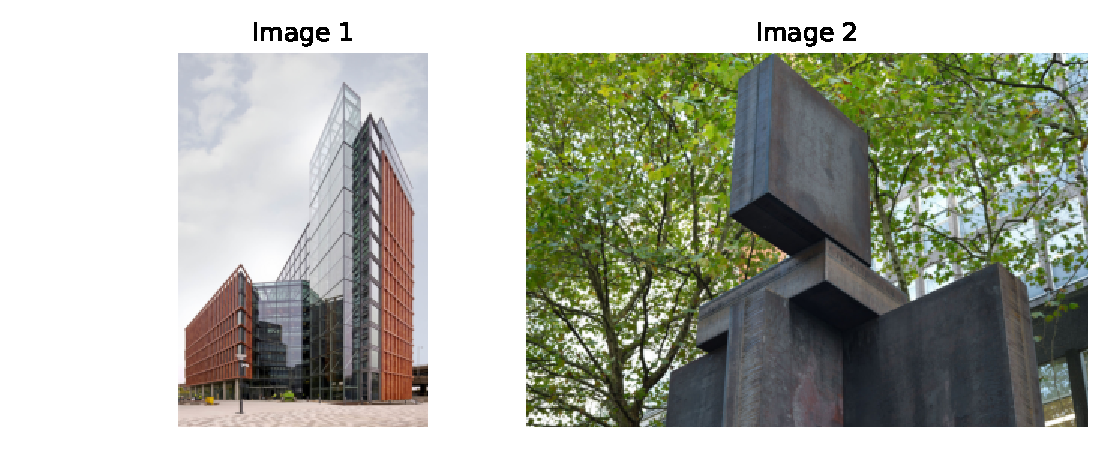
\includegraphics[width=0.9\textwidth]{../img/ex1_original_images.pdf}
    \end{figure}

\bblue{Histograms}
    \begin{figure}
        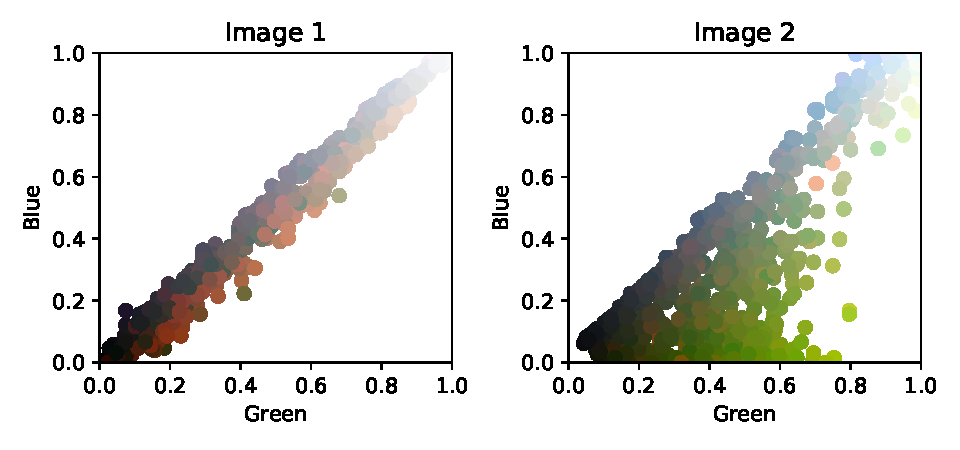
\includegraphics[width=0.9\textwidth]{../img/ex1_colour_histograms.pdf}
    \end{figure}
    
\end{minipage}
\hfill
\begin{minipage}{0.56\textwidth}
\qquad\bblue{Transported images}
    \begin{figure}
        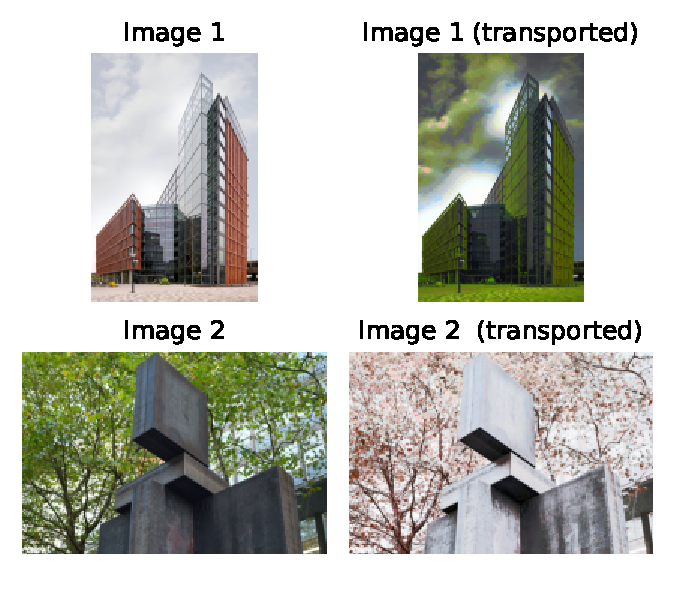
\includegraphics[width=0.99\textwidth]{../img/ex1_result.pdf}
    \end{figure}
\end{minipage}

\begin{textblock}{0.45}(0.01,0.56)
\small
\bred{
\underline{
    Notebook: \href{https://github.com/felipe-tobar/OT-tutorial-MLSP-2024/blob/main/Codes/Colour_transfer.ipynb}{Colour\_transfer.ipynb}
}}
\end{textblock}
\end{frame}


\begin{frame}{\bred{Motivation:}  Domain  adaptation}

\begin{minipage}{0.49\textwidth}
\vspace{1em}
\bblue{Same tasks, different domains}
    \begin{figure}
        \includegraphics[trim={1.5cm 20.5cm 2cm 1.5cm},clip, page=2, width=0.9\textwidth]{../img/OT4DA}\hfill
    \end{figure}
\vspace{-0.5em}
    \begin{figure}
        \includegraphics[trim={1cm 21.5cm 10cm 2cm},clip, page=3, width=0.9\textwidth]{../img/OT4DA}
    \end{figure}
\end{minipage}
\hfill
\begin{minipage}{0.49\textwidth}

    \begin{figure}
        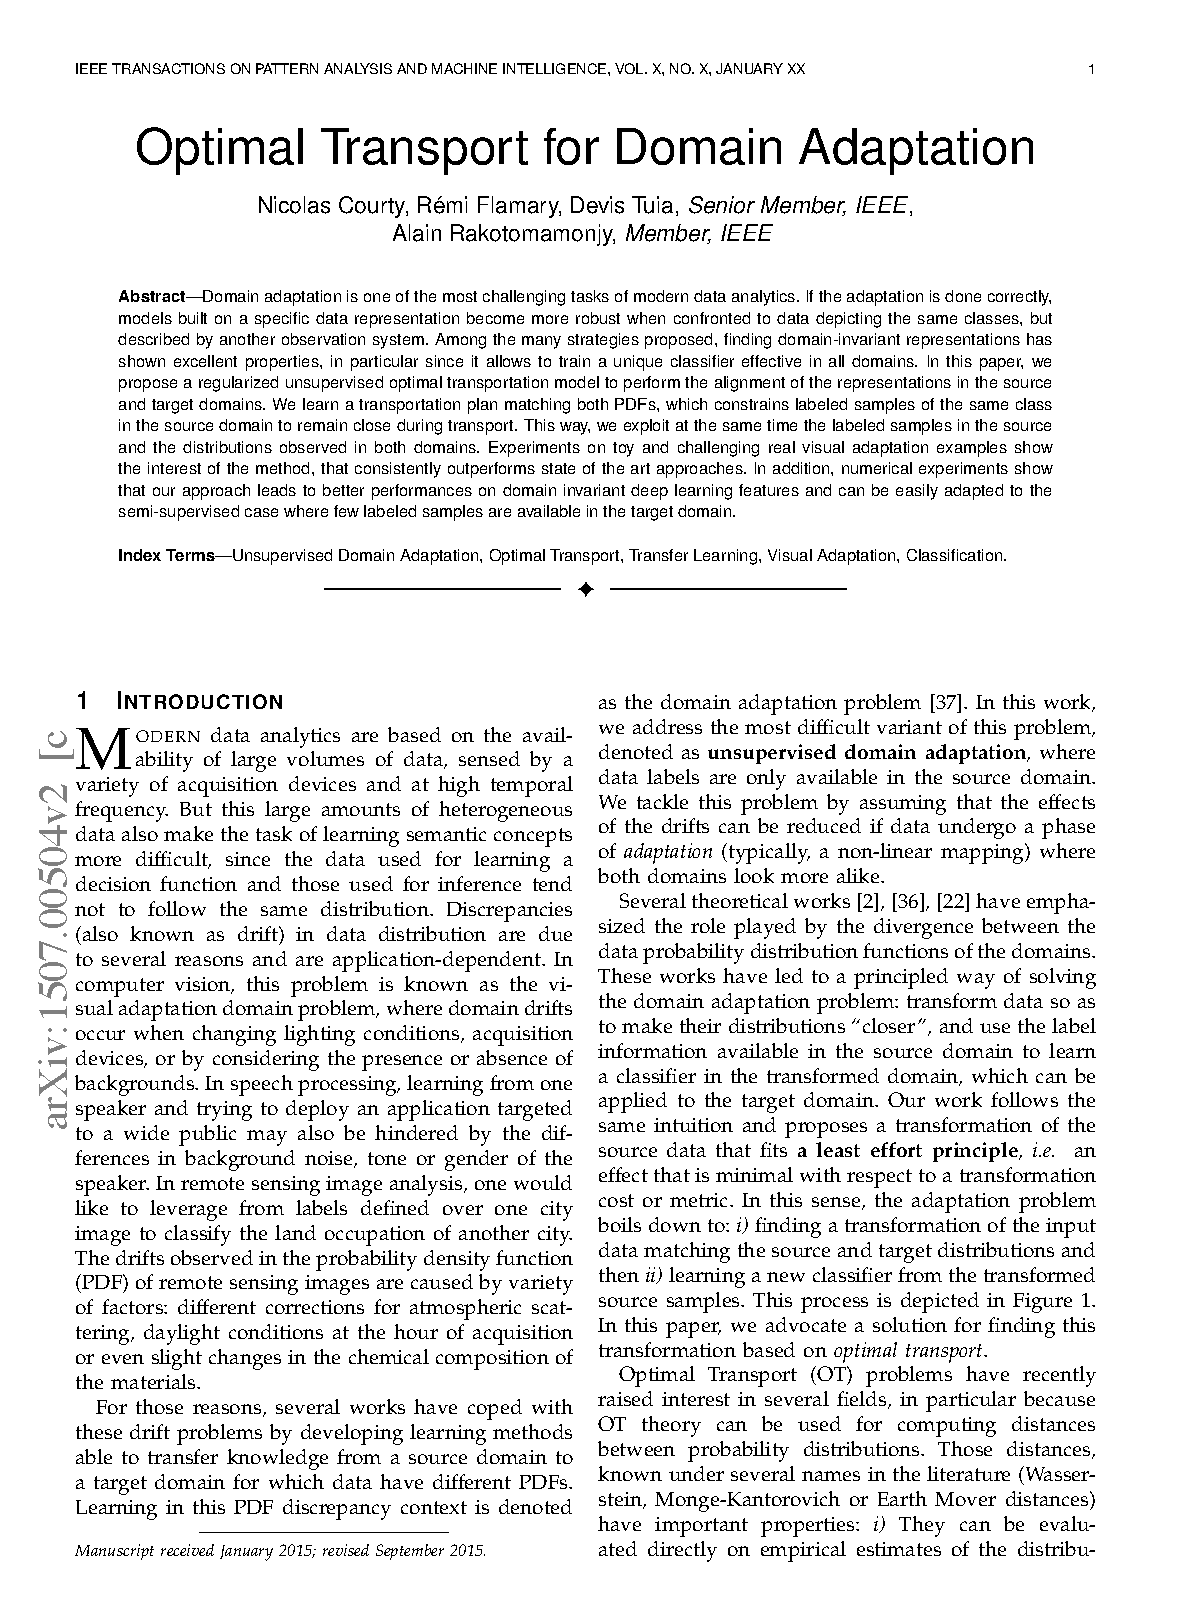
\includegraphics[trim={0cm 18.5cm 0cm 0cm},clip, page=1, width=0.95\textwidth]{../img/OT4DA}
    \end{figure}

{
\tiny
Nicolas Courty, Rémi Flamary, Devis Tuia, Alain Rakotomamonjy. Optimal Transport for Domain
Adaptation. \emph{IEEE Transactions on Pattern Analysis and Machine Intelligence} 2016, 39 (9), pp.1853-
1865.
}

\end{minipage}




\begin{textblock}{0.45}(0.56,0.54)
\small
\bred{
\underline{
    Link: \href{https://arxiv.org/abs/1507.00504}{arxiv.org/abs/1507.00504}
}}
\end{textblock}
\end{frame}





\begin{frame}{\bred{Example 4:} Domain adaptation}

\begin{minipage}{0.49\textwidth}
\vspace{1em}
\bblue{Two datasets: same task}
    \begin{figure}
        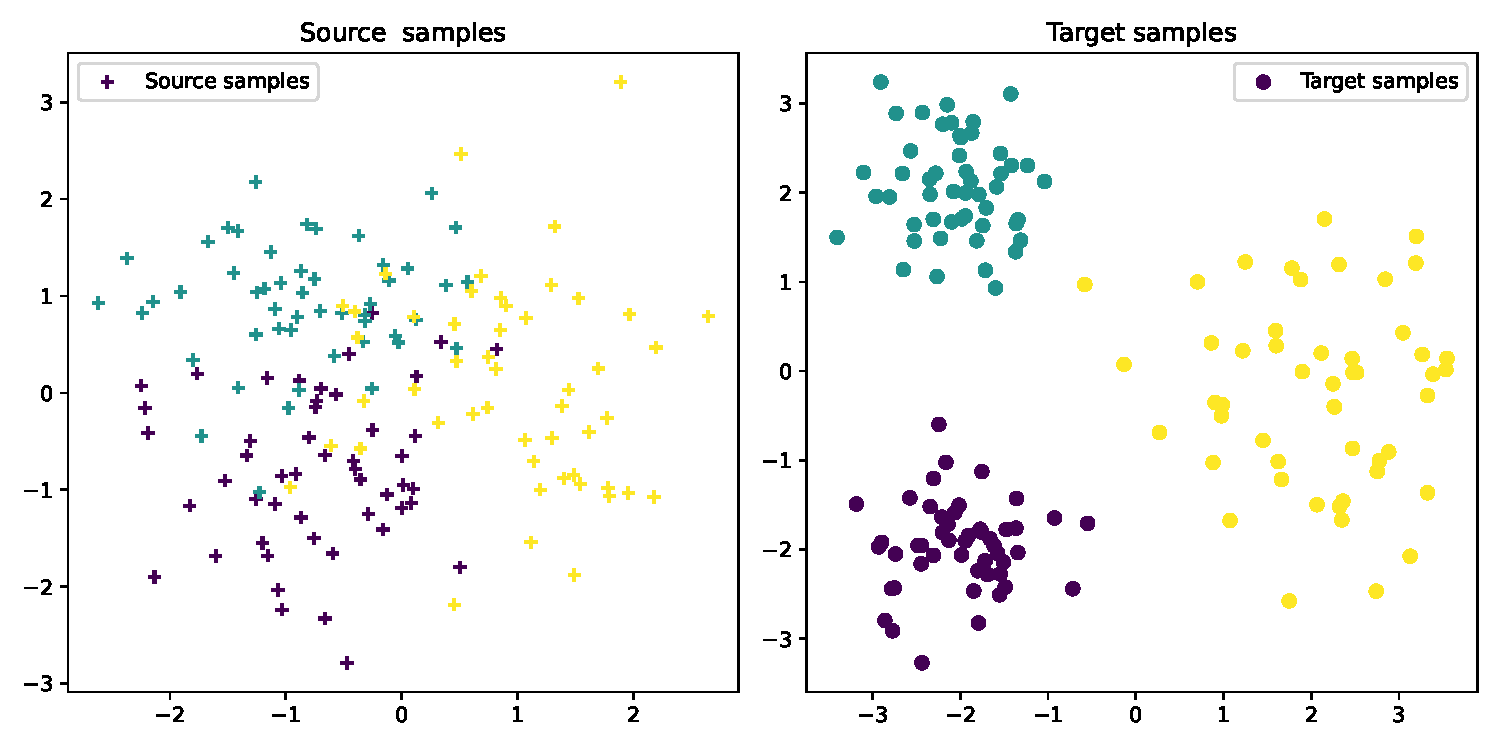
\includegraphics[width=0.78\textwidth]{../img/DA_original_samples.pdf}
    \end{figure}
\vspace{-0.5em}
\bblue{Transport}
    \begin{figure}
        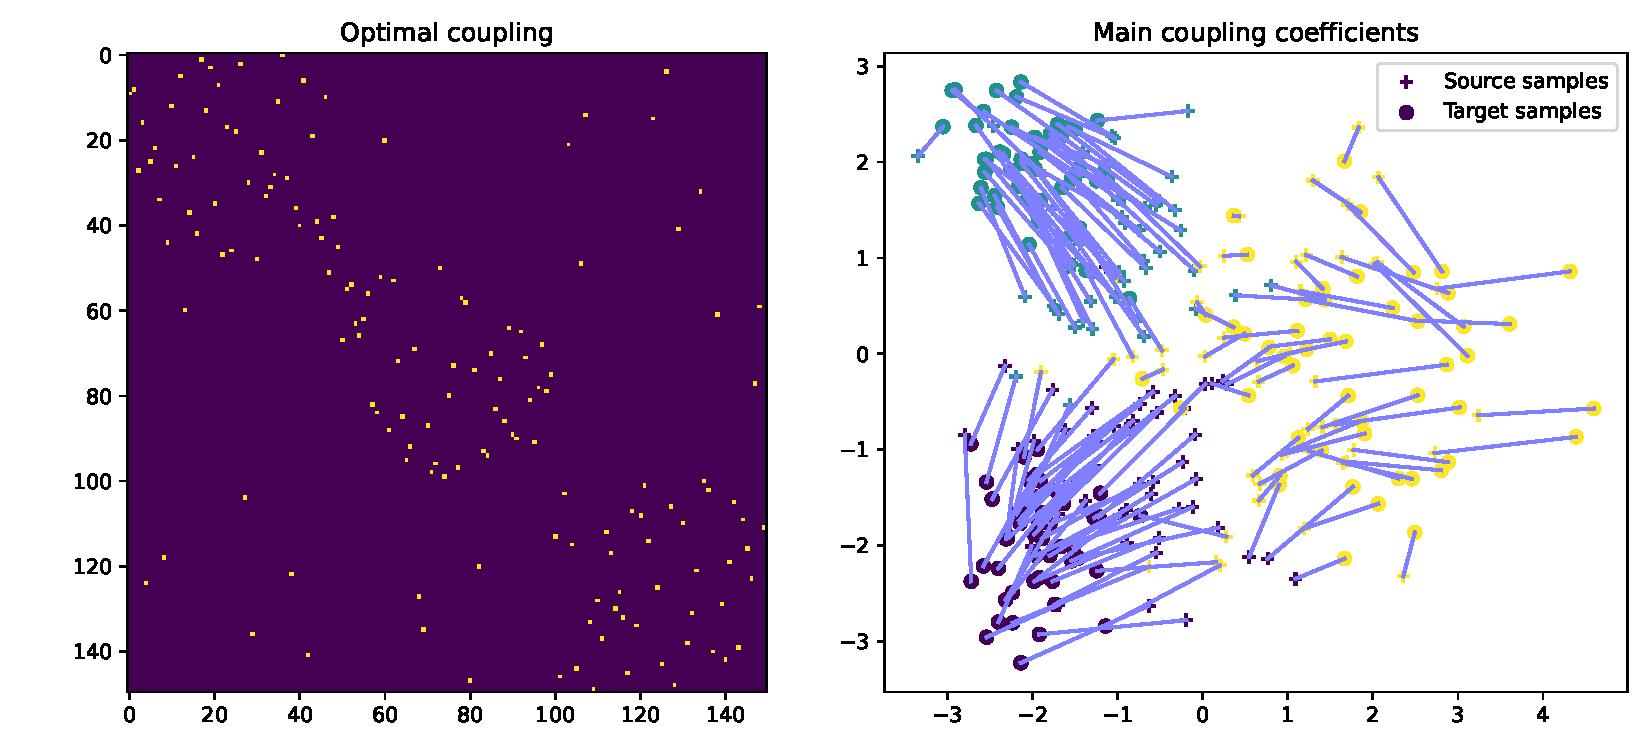
\includegraphics[width=0.85\textwidth]{../img/DA_coupling.pdf}
    \end{figure}
    
\end{minipage}
\hfill
\begin{minipage}{0.49\textwidth}
\bblue{Domain: adapted}
    \begin{figure}
        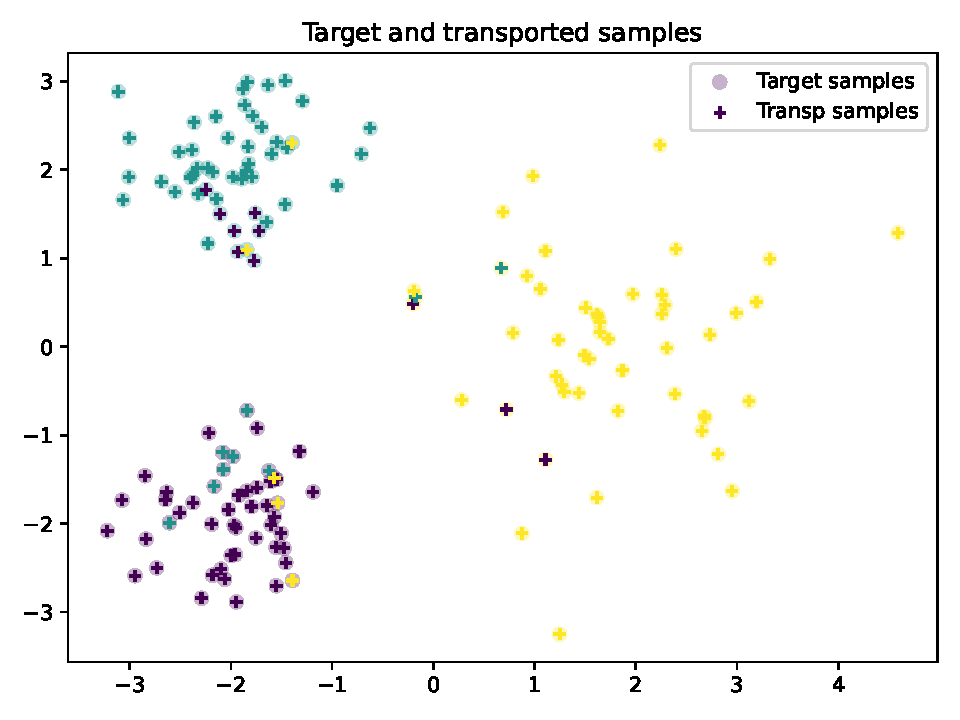
\includegraphics[width=0.9\textwidth]{../img/DA_samples.pdf}
    \end{figure}
\end{minipage}

\begin{textblock}{0.45}(0.56,0.54)
\small
\bred{
\underline{
    Notebook: \href{https://github.com/felipe-tobar/OT-tutorial-MLSP-2024/blob/main/Codes/Domain_adaptation.ipynb}{Domain\_adaptation.ipynb}
}}
\end{textblock}
\end{frame}







\begin{frame}{Remarks} 
    \begin{itemize}
        \item We've been using the cost $c(x,y) = |x-y|^p, p\geq 1$. Then, if $\mu$ and $\nu$ are absolutely continuous wrt the Lebesgue measure, the Kantorovich problem as a unique solution. Furthermore, this solution is the same solution of the Monge problem.
        \item If $p=2$, the optimal map is the gradient of a convex function
        \item In some cases the optimal plan will require to split mass (e.g., in the case of atomic measures) and thus Monge's solution may fail to exist. 
        \item Luckily, from a (Kantorovich) transport plan we can always extract a transport map, e.g., via the barycentric projection
    \end{itemize}
\end{frame}






\begin{frame}{Solving discrete OT}

Let $\er{\mu}=\sum_{i=1}^n\delta_{x_i}$ and $\eb{\nu}=\sum_{j=1}^m\delta_{y_j}$
\begin{block}{}
$$\pi^\ast \in \underset{\pi\in\Pi(\er{\mu},\eb{\nu})}{\argmin} \ \langle C, \pi \rangle$$
\end{block}

{\vspace{0.3cm}\begin{itemize}
\item[$\bullet$] Linear problem: it can be rewritten in a vectorial form $\min_{t\geq 0} F(t) = c^Tt$
\item[$\bullet$] Linear constraints of the form $\pi\mathds{1}_m =\er{\mu}$ and $\pi^T\mathds{1}_n=\eb{\nu}$
\end{itemize}
\vspace{0.1cm}$\Longrightarrow$ Linear problem + linear constraints: complexity is $\mathcal{O}(n^3\log(n))$}

{\vspace{0.3cm}$\Longrightarrow$ Need for solvers that provide approximate solutions! See [Peyré et Cuturi 2019]}
\end{frame}

\begin{frame}{Regularization of OT}
\begin{block}{}
$$\pi_{\varepsilon} = \argmin_{\pi\in\R^{n\times m}_+} \ \langle C,\pi\rangle + \varepsilon\ \Omega(\pi)$$
\end{block}

\vspace{0.2cm}Advantages of regularizing the optimisation problem:
\begin{itemize}
\item[$\bullet$] Fast and \emph{smoother} solutions
\item[$\bullet$] Encoding task's prior knowledge
\item[$\bullet$] Better posed problem (convexity, stability).
\end{itemize}
\vspace{1em}

Regularisation functionals
\begin{itemize}
\item[$\bullet$] Entropic regularization [Cuturi, 2013]
\item[$\bullet$] KL, Itakura Saito, $\beta$-divergences, [Papadakis \& Papadakis, 2018]
\end{itemize}

\end{frame}



\begin{frame}{Entropy regularized OT [Cuturi, 2013]}
\begin{block}{}
The solution of 
$$\OT(\er{\mu},\eb{\nu}) = \min_{\pi\in\Pi(a,b)} \ \langle C,\pi\rangle + \varepsilon \sum_{i,j} \pi_{ij}\log(\pi_{ij})$$
is of the form
$$\pi_\varepsilon^* = \diag(u)\exp\left(-\frac{C}{\varepsilon}\right)\diag(v)$$
where $u$ and $v$ follow an alternating recursive formula. 
\end{block}
\begin{minipage}{0.5\textwidth}
   {\vspace{0.3cm}
\begin{itemize}
\item[$\bullet$] From Sinkhorn theorem [Sinkhorn, 1964], we know that $\diag(u)$ and $\diag(v)$ exist and are unique.
\item[$\bullet$] Sinkhorn-Knopp algorithm [Knight, 2008] allows to solve it efficiently
\end{itemize}} 
\end{minipage}
\hfill
\begin{minipage}{0.49\textwidth}
\centering
        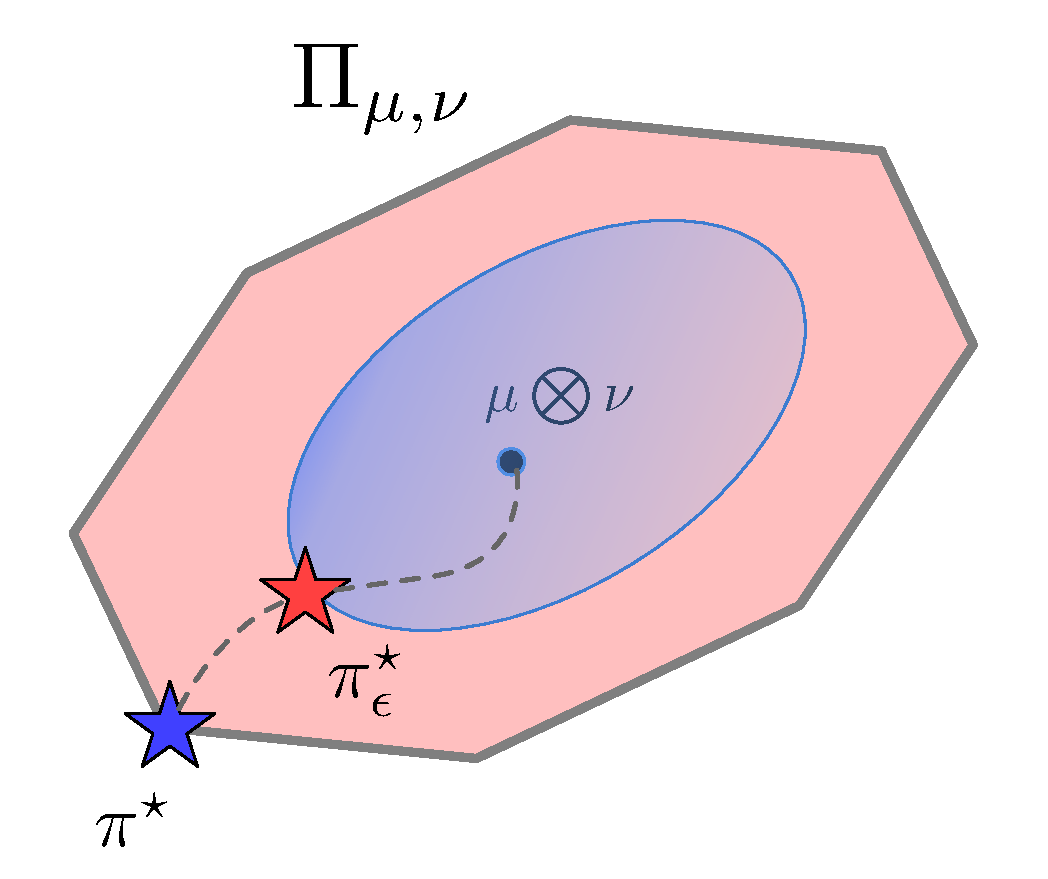
\includegraphics[width=0.6\textwidth]{../img/polytope2.pdf}\hspace{2em}
\end{minipage}



\end{frame}




\begin{frame}{\bred{Example 5:} Sinkhorn regularisation and effect}

\begin{minipage}{0.49\textwidth}  
\begin{figure}
        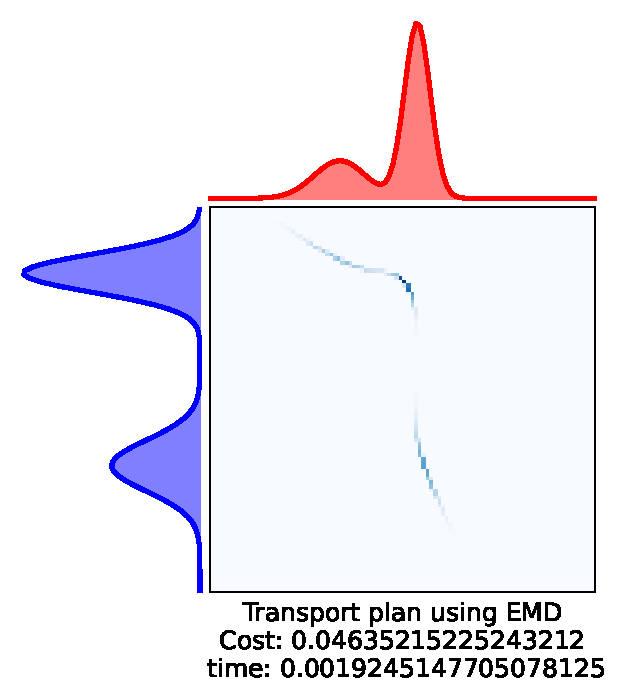
\includegraphics[width=0.8\textwidth]{../img/EMD_vs_S1.pdf}\hspace{2em}
    \end{figure}
\end{minipage}
\hfill
\begin{minipage}{0.49\textwidth}
\begin{figure}
        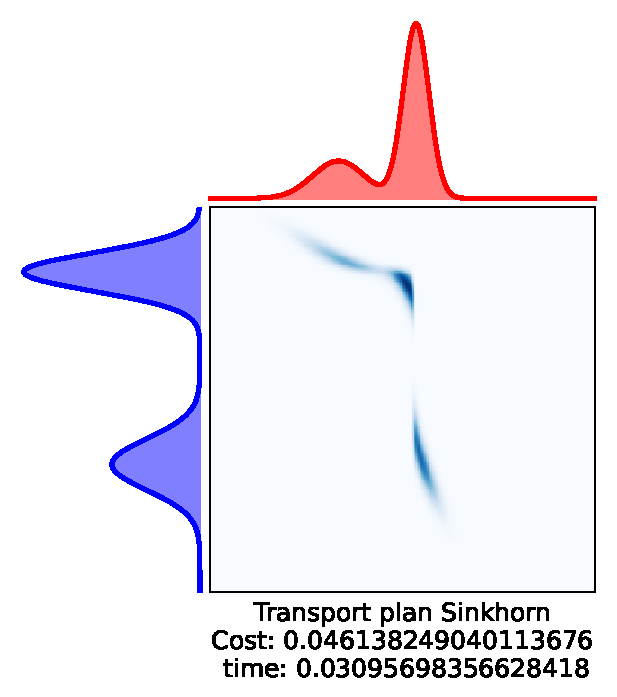
\includegraphics[width=0.8\textwidth]{../img/EMD_vs_S2.pdf}\hspace{2em}
    \end{figure}
\end{minipage}

\begin{textblock}{0.45} (0.62,0.54)
\small
\bred{
\underline{
    Notebook: \href{https://github.com/felipe-tobar/OT-tutorial-MLSP-2024/blob/main/Codes/sinkhorn.ipynb}{sinkhorn.ipynb}
}}
\end{textblock}
\end{frame}





\section{Part II\\ The Wasserstein distance and metric properties}



\begin{frame}
    \Large \bblue{Part II\\ The Wasserstein distance and metric properties}
\end{frame}




\begin{frame}{OT \emph{lifts} a distance from the measures' support}
    \bred{A family of distances between measures}\\
    \begin{minipage}{0.59\textwidth}
        The \bblue{Kantorovitch problem}
        \begin{equation*}
            P^\star \in \inf_{P\in\Pi_{\mu,\nu}} \langle P , C\rangle = \sum_{i,j}^{n,m} C_{ij}P_{ij} 
        \end{equation*}
        allows defining the \bblue{Wasserstein distance} of order $p$
        \begin{equation*}
            W^p_p(\mu, \nu) =  \langle P^\star , C\rangle
        \end{equation*}
        where the moving cost $c(x, y) = {d(x, y)}^p = \| x - y \|^p$.\\
        It is often depicted as an ``horizontal'' distance
\begin{itemize}
          \item[\bred{$\checkmark$}] \bblue{symmetry}
          \item[\bred{$\checkmark$}] \bblue{identity of indiscernibles} 
          \item[\bred{$\checkmark$}] \bblue{triangular inequality}
      \end{itemize}       
    \end{minipage}
    \hfill
    \begin{minipage}{0.4\textwidth}
    \begin{figure}
        \centering
            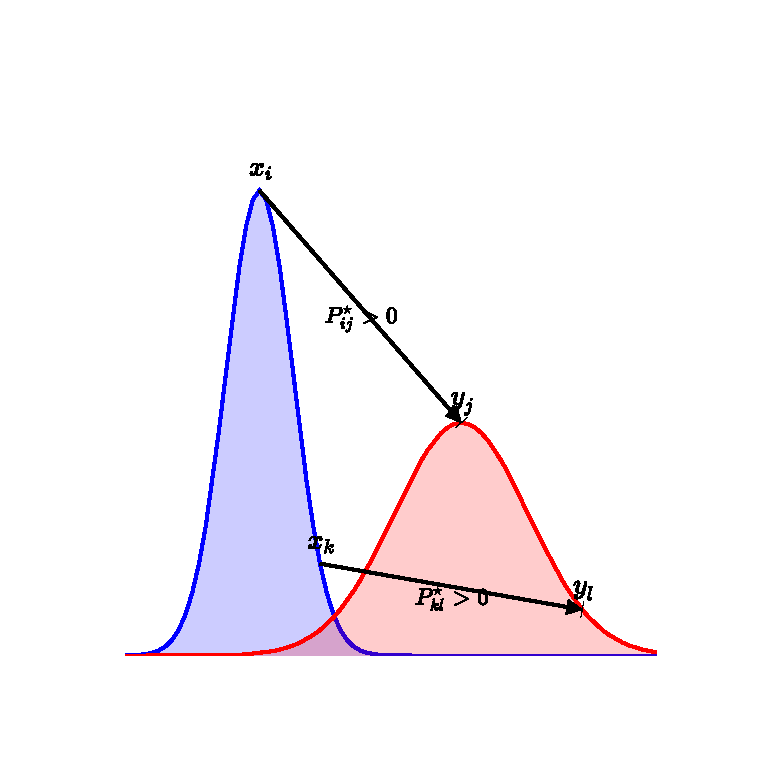
\includegraphics[trim={2cm 2cm 2cm 2cm},clip, width=0.9\textwidth]{../img/horizontal_distance.pdf}
        \end{figure}
        \centering
        \small
    \bred{
    \underline{
        Notebook: \href{https://github.com/felipe-tobar/OT-tutorial-MLSP-2024/blob/main/Codes/Horizontal distance.ipynb}{Horizontal distance.ipynb}
    }}
    \end{minipage}
    
    %We need a distance, OT provides one. Show how some \emph{strong} topologies cannot be used for learning systems
\end{frame}

\begin{frame}{The Wasserstein distance (vs others)}
    \begin{itemize}
        \item Does not need overlapping support (as KL)
        \item Determines the \emph{degree of dissimilarity} between distributions
    \end{itemize}
    \begin{figure}
        \centering
            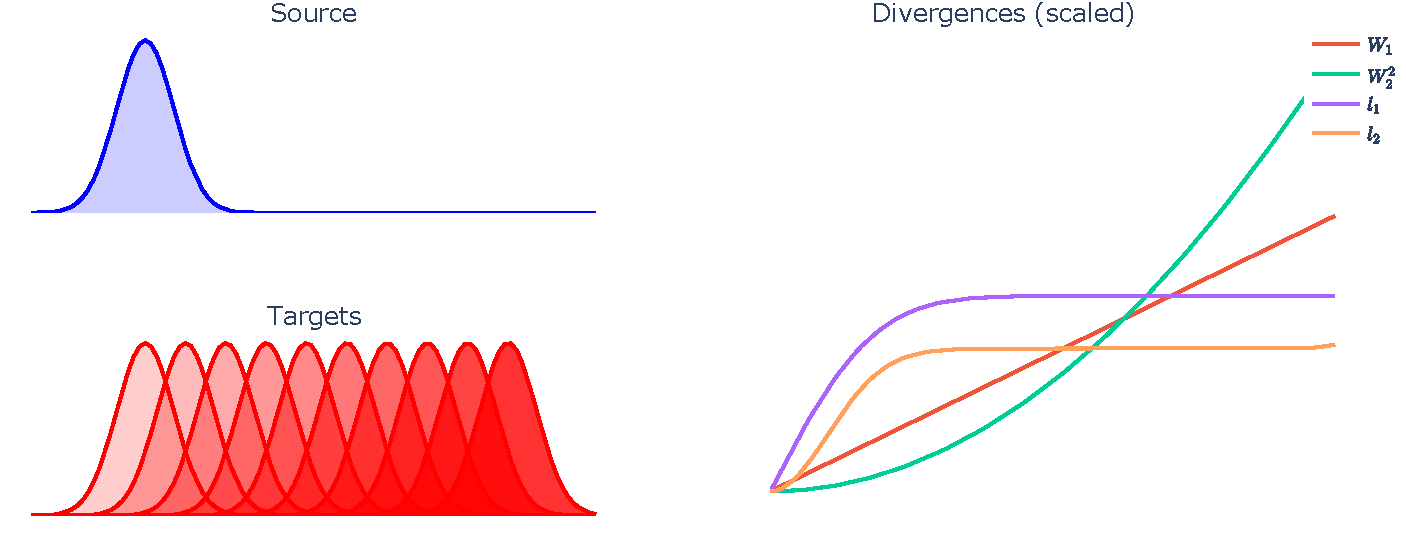
\includegraphics[trim={0 0 0 0},clip, width=0.7\textwidth]{../img/wasserstein_1d.pdf}
        \end{figure}
        \centering
        \small
    \bred{
    \underline{
        Notebook: \href{https://github.com/felipe-tobar/OT-tutorial-MLSP-2024/blob/main/Codes/Wasserstein distance.ipynb}{Wasserstein\_distance.ipynb}
    }}

\end{frame}

\begin{frame}{On the suitability of $W_p$ for learning}

\begin{itemize}
    \item Thus far, we have referred to \emph{spaces of probability functions}, but we are interested in applying $W_p$ on spaces of \bred{generative models}.
    \item Learning in such a space requires, more than a distance, a notion of \bred{convergence}
    \item Consider $\mu_\text{data}$ to be the true data distribution. We want to find a model $(P_\theta)_{\theta\in\Theta}$ such that $P_\theta \to \mu_\text{data}$, or equivalently, $D(\mu_\text{data},P_\theta)\to 0$ --- for a \bblue{reasonable} divergence $D$.
\end{itemize}
\vspace{2em}
\centerline{\bblue{Discussion:} Consider $\delta_{x_0}$ and $\delta_{x_i}, x_i\to x_0$}
\vspace{2em}

\centerline{OT allows for \bred{assessing} convergence and \bred{constructing} convergent sequences}

\end{frame}



\begin{frame}{\bred{Example 6:} Gradient flows on Wasserstein space}
    \bblue{Wasserstein space $\mathbb{W}_p$:} space endowed with the distance $W_p$
    \begin{itemize}
        \item In the space $\mathbb{W}_p(\mathbb{R}^d)$, we have $W_p(\mu_n, \mu) \to 0$ iff $\mu_n \to \mu$ (weak topology)
    \end{itemize}
    \bblue{Consider the loss $W_2^2(\mu_t, \mu)$.} The figure below shows how a distribution $\mu_0$ evolves under de application of gradient flow of this loss.
    \begin{figure}
        \centering
            \only<1>{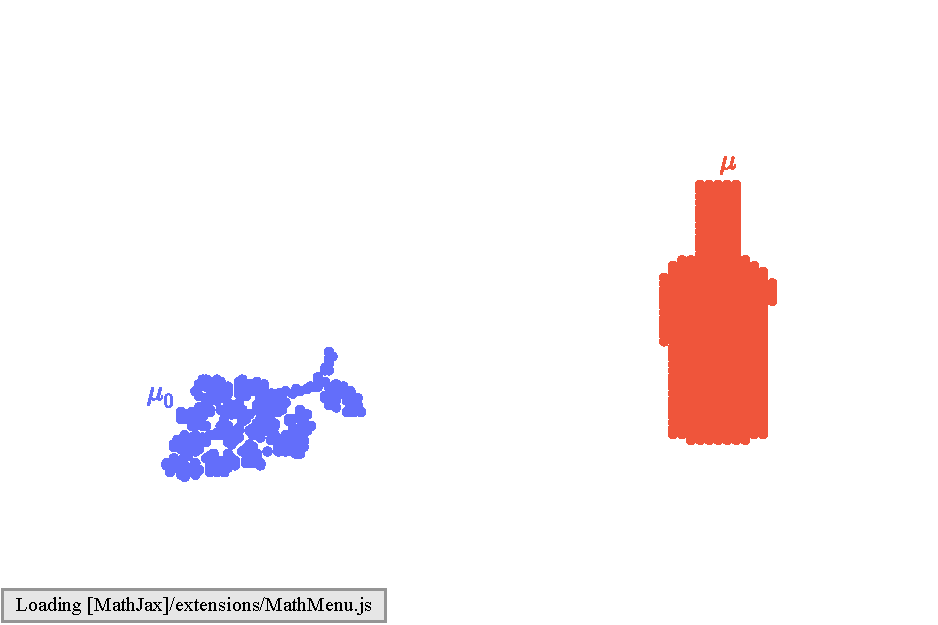
\includegraphics[trim={2cm 2cm 2cm 2.5cm},clip, width=0.6\textwidth]{../img/GF_init.pdf}}
            \only<2>{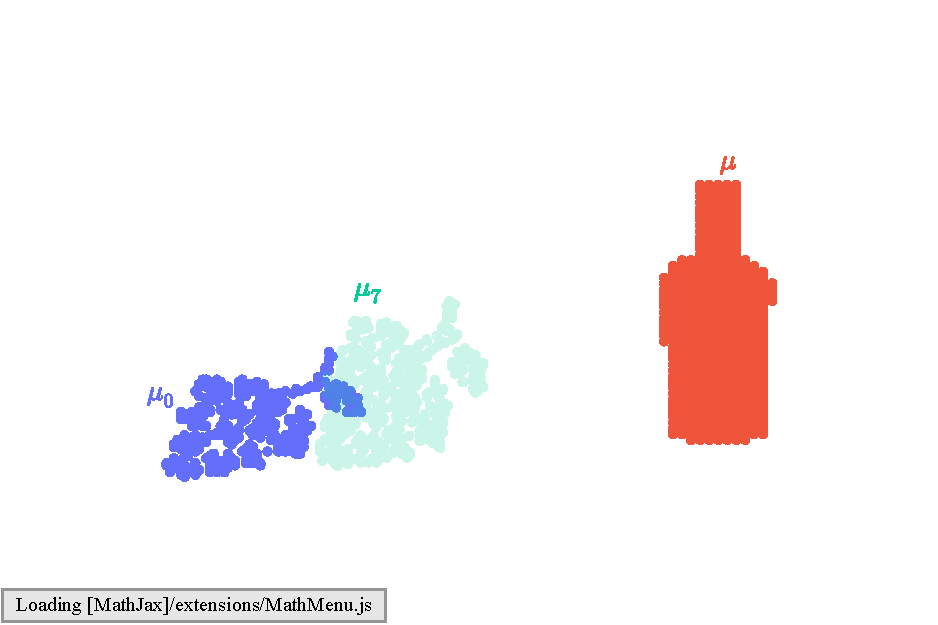
\includegraphics[trim={2cm 2cm 2cm 2.5cm},clip, width=0.6\textwidth]{../img/GF_step1.pdf}}
            \only<3>{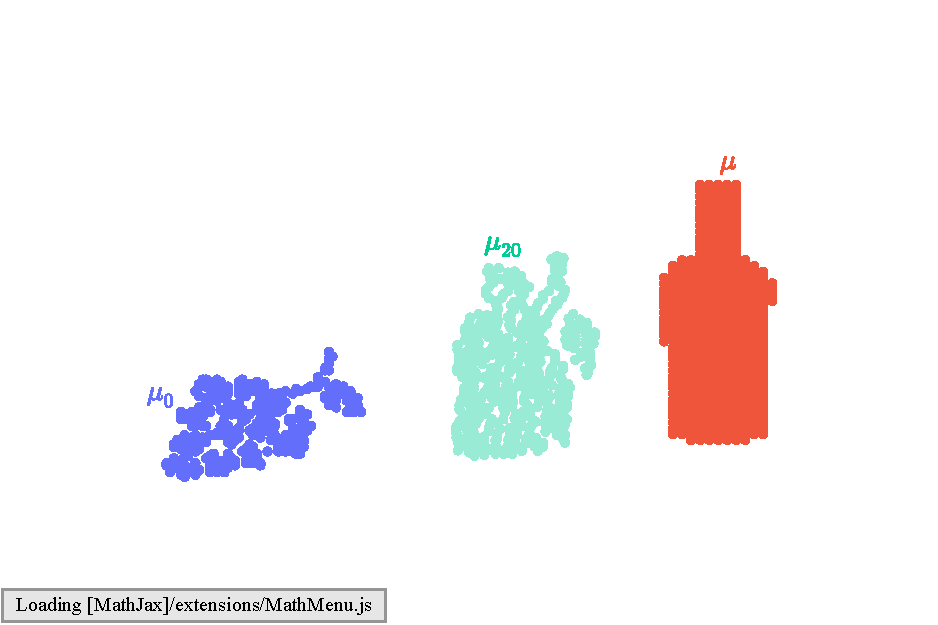
\includegraphics[trim={2cm 2cm 2cm 2.5cm},clip, width=0.6\textwidth]{../img/GF_step2.pdf}}
            \only<4>{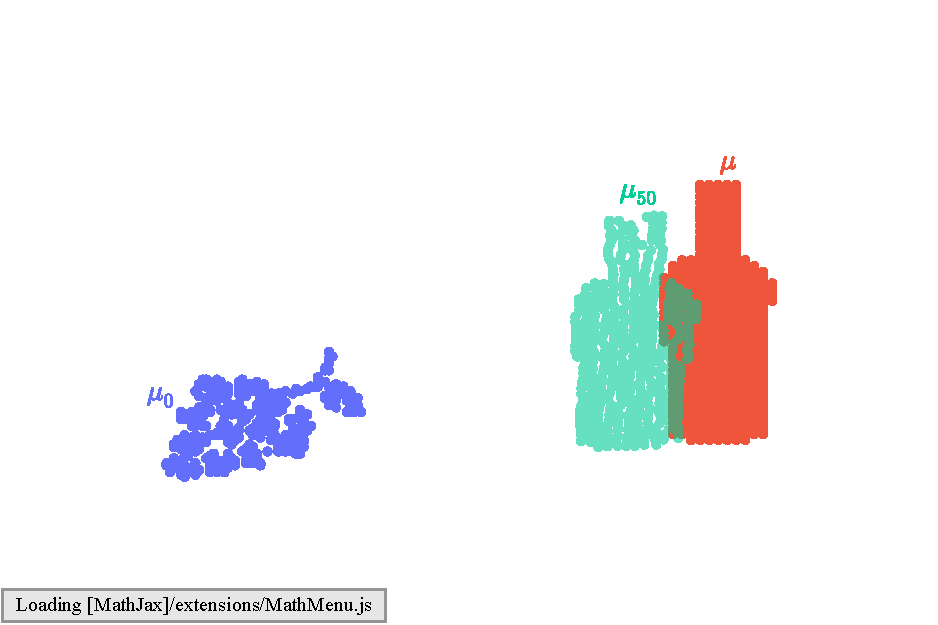
\includegraphics[trim={2cm 2cm 2cm 2.5cm},clip, width=0.6\textwidth]{../img/GF_step3.pdf}}
            \only<5>{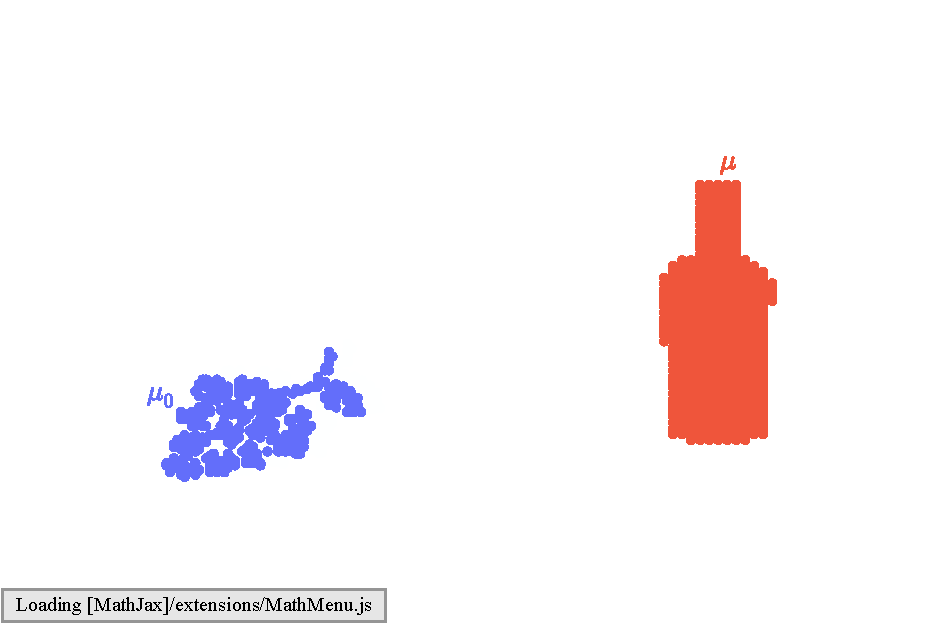
\includegraphics[trim={2cm 2cm 2cm 2.5cm},clip, width=0.6\textwidth]{../img/GF_final.pdf}}            
        \end{figure}
        \bred{
    \underline{
        \centering
        Notebook: \href{https://github.com/felipe-tobar/OT-tutorial-MLSP-2024/blob/main/Codes/Wasserstein Gradient Flows.ipynb}{Wasserstein Gradient Flows.ipynb}
    }}
\end{frame}



\begin{frame}{Geodesic paths between distributions}
    \begin{minipage}{0.59\textwidth}
    A geodesic generalizes the concept of a straight line between two points\\
    \begin{figure}
        \centering
            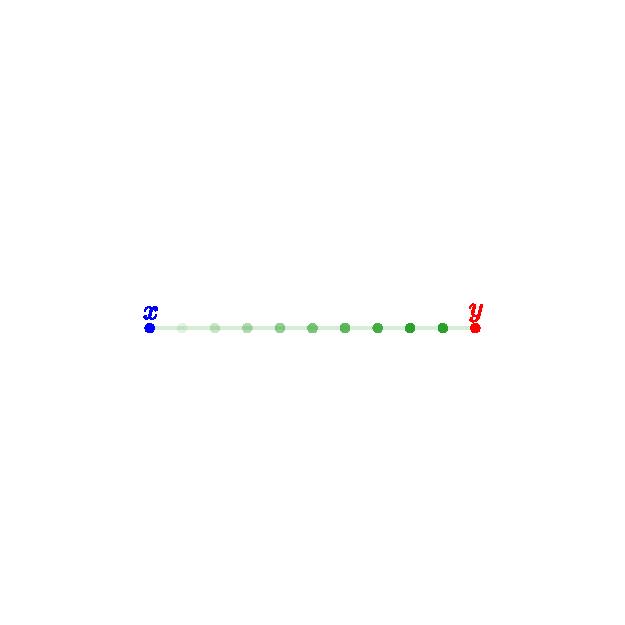
\includegraphics[trim={2cm 4.5cm 2cm 5cm},clip, width=0.7\textwidth]{../img/straightLine.pdf}
        \end{figure}

    It is a curve that represents the shortest path between two manifolds\\
    Euclidean space with a $l_2$ distance is a \bred{geodesic space}\\
    \begin{equation*}
        \forall t \in [0,1],\quad \mu^{1\to 2}(t) = t\mu_2 + (1-t) \mu_1
    \end{equation*} 
    Allows ``vertical'' interpolation between the distributions
\end{minipage}
\hfill
\begin{minipage}{0.4\textwidth}

        \begin{figure}
            \centering
                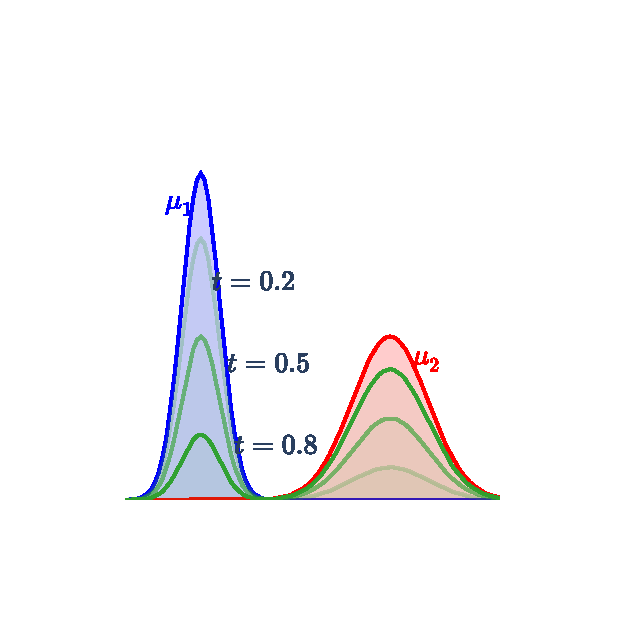
\includegraphics[trim={2cm 2cm 2cm 2cm},clip, width=1\textwidth]{../img/geodesic_Euc_1d.pdf}
            \end{figure}
\end{minipage}

\vspace{2em}
        \small
\bred{\underline{
        Notebook: \href{https://github.com/felipe-tobar/OT-tutorial-MLSP-2024/blob/main/Codes/Wasserstein Geodesics.ipynb}{Wasserstein Geodesics.ipynb}
    }}
\end{frame}

\begin{frame}{Geodesic properties of the Wasserstein space}
    \begin{minipage}{0.59\textwidth}
    $\mathbb{W}_p$ is a \bred{geodesic space}
    \begin{itemize}
        \item Given a Monge map $T$ between $\mu_1$ and $\mu_2$ such that $T_{\#}\mu_1 = \mu_2$, a geodesic curve $\mu^{1\to 2}$ is
        \begin{equation*}
\forall t \in [0,1],\quad \mu^{1\to 2}(t) = {(t T + (1-t)\text{Id})}_{\#} \mu_1
        \end{equation*} 
        \item It represents the shortest path (on the Wasserstein space $\mathbb{W}_p$) between $\mu_1$ and $\mu_2$
        \item Allows ``horizontal'' interpolation between the distributions
    \end{itemize}
\end{minipage}
\hfill
\begin{minipage}{0.4\textwidth}
    \begin{figure}
        \centering
            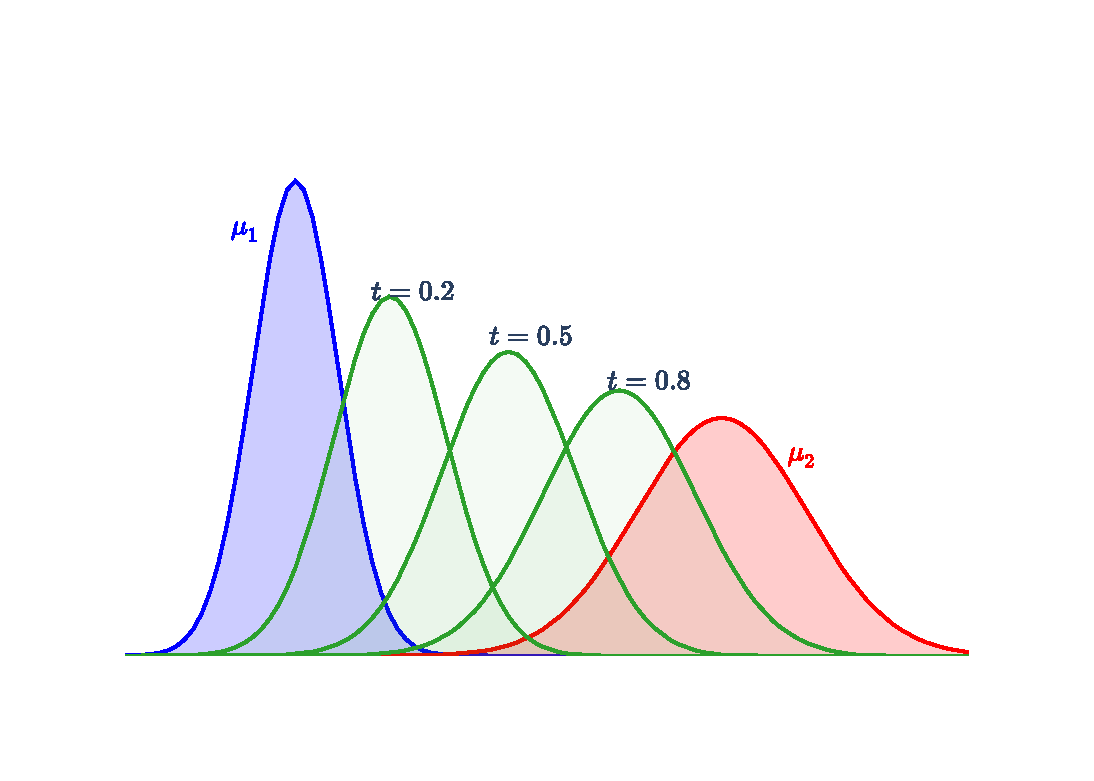
\includegraphics[trim={2cm 2cm 2cm 2cm},clip, width=1\textwidth]{../img/geodesic_1d.pdf}
        \end{figure}
\end{minipage}

\vspace{2em}
        \small
\bred{\underline{
        Notebook: \href{https://github.com/felipe-tobar/OT-tutorial-MLSP-2024/blob/main/Codes/Wasserstein Geodesics.ipynb}{Wasserstein Geodesics.ipynb}
    }}
\end{frame}





\begin{frame}[plain]{The Wasserstein barycentre}

    Given a set of distributions $\mu_s$, compute: 
    \begin{equation*}
        \overline{\mu} = \arg \min_{\mu} \sum_{i=1}^s \lambda_i W^p_p(\mu, \mu_i)
    \end{equation*}
    where $\lambda_i > 0$ and $\sum_{i=1}^s \lambda_i  = 1$.\vspace{0.5em}

    Generalizes the interpolation between more than 2 measures.\\
    For discrete measures $\mu = \sum_{i=1}^n a_i \delta_{x_i}$ $\Rightarrow$ we can fix the weights $a_i$ and/or the support $x_i$.
    \only<1>{\begin{figure}
        \centering
            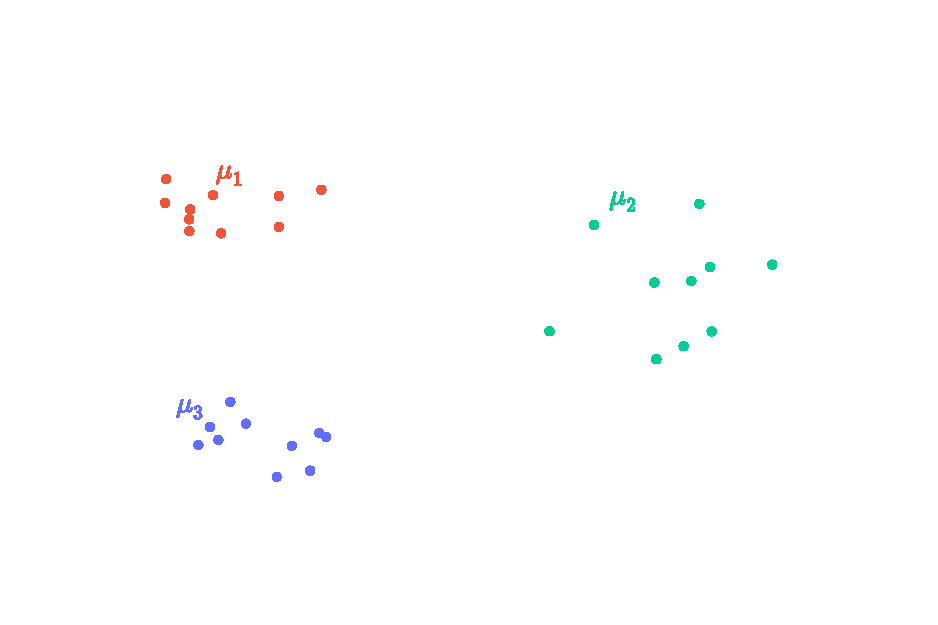
\includegraphics[trim={2cm 2cm 2cm 2cm},clip, width=0.45\textwidth]{../img/distrib_bary.pdf}
        \end{figure}
        }
        \only<2>{\begin{figure}
            \centering
                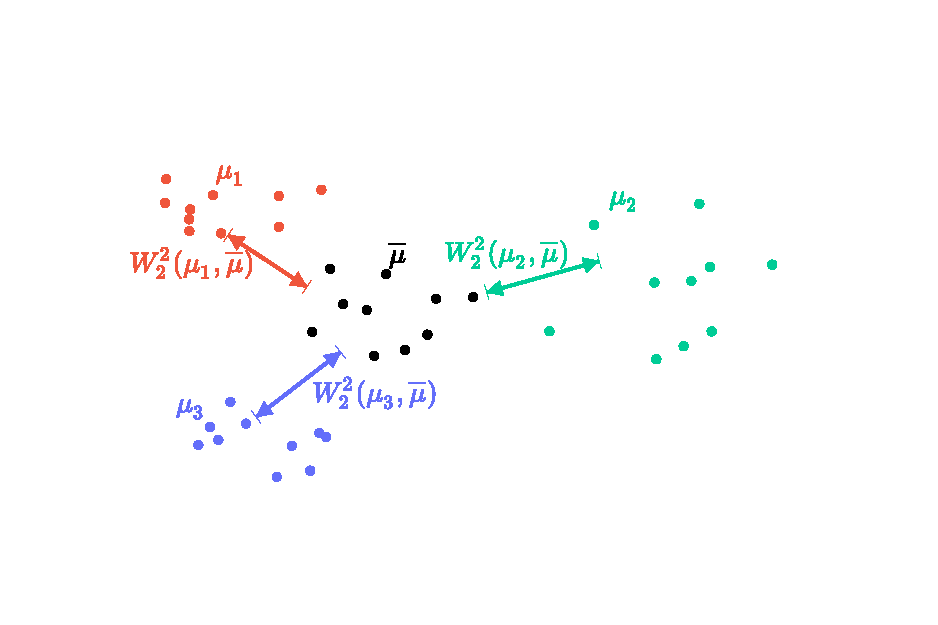
\includegraphics[trim={2cm 2cm 2cm 2cm},clip, width=0.45\textwidth]{../img/barycenter_2d.pdf}
            \end{figure}
            }
            \begin{textblock}{0.45}(0.56,0.54)
        \bred{
            \small
            \underline{Notebook: \href{https://github.com/felipe-tobar/OT-tutorial-MLSP-2024/blob/main/Codes/Wasserstein barycenter.ipynb}{Wasserstein barycenter.ipynb}
            }}
            \end{textblock}
\end{frame}

\begin{frame}[plain]{The Wasserstein barycentre}
    \bred{Example on averaging over images} \\
    \begin{minipage}{0.48\textwidth}
        
    \begin{figure}
        \centering
            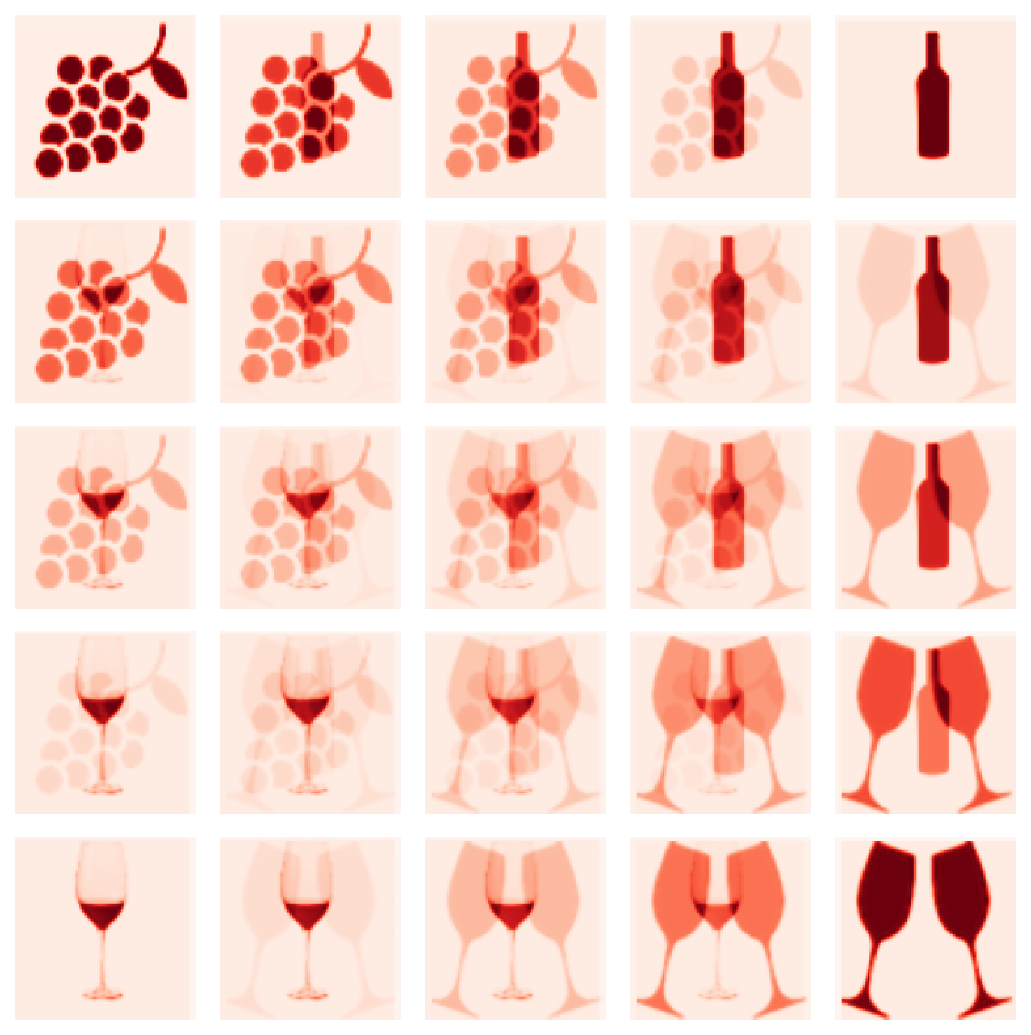
\includegraphics[clip, height=0.7\textheight]{../img/symboles_wine_L2.pdf}
            \caption{In the \bblue{Euclidean} space }
        \end{figure}
        
    \end{minipage}
    \hfill
    \begin{minipage}{0.48\textwidth}
\begin{figure}
            \centering
                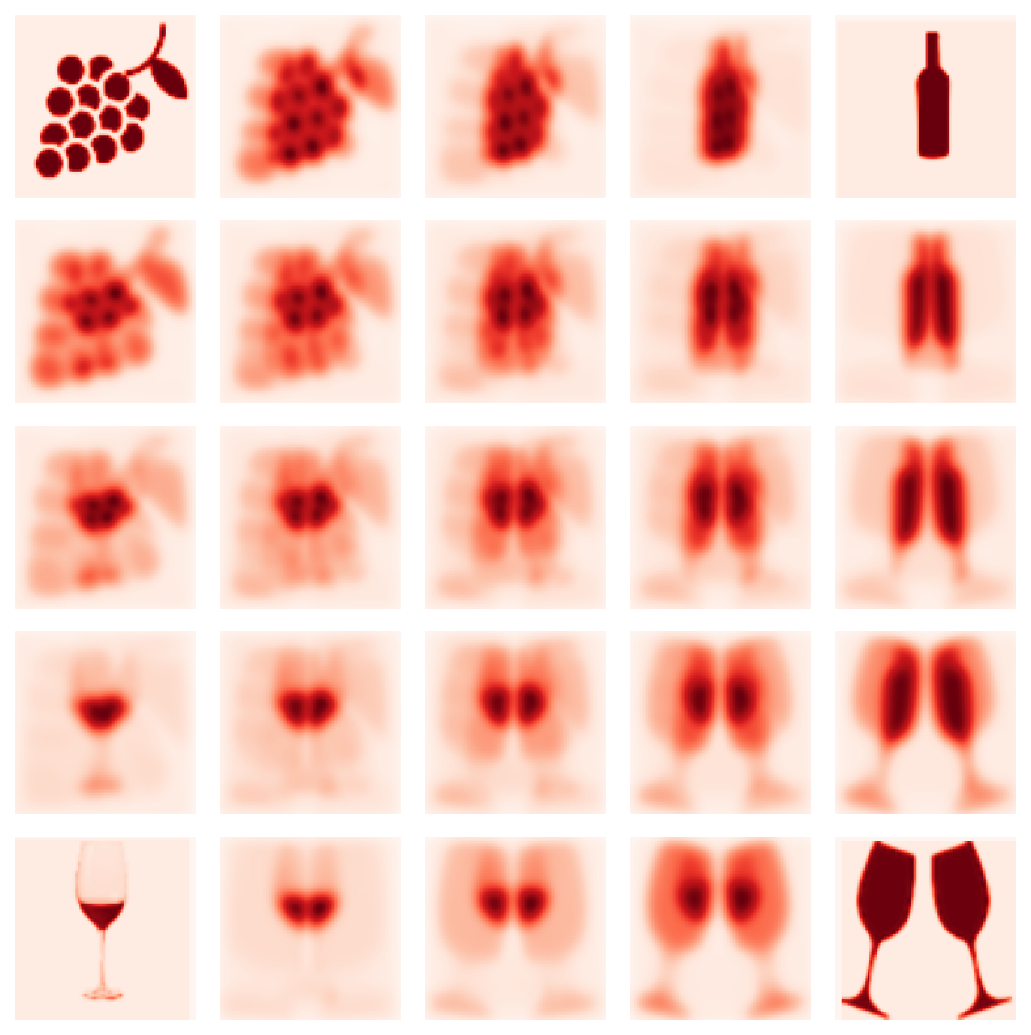
\includegraphics[clip, height=0.7\textheight]{../img/symboles_wine_bary.pdf}
            \caption{In the \bblue{Wasserstein} space}
            \end{figure}
            
        \end{minipage}
        \bred{
            \underline{
                Notebook: \href{https://github.com/felipe-tobar/OT-tutorial-MLSP-2024/blob/main/Codes/Wass bary 4 distribs.ipynb}{Wass bary 4 distribs.ipynb}
            }}
\end{frame}

\section{Part III \bred{(if time allows)}\\ OT for time series: The Wasserstein-Fourier distance}



\begin{frame}
\centerline{\bred{(if time allows)}}
\vspace{2em}
    \Large \bblue{Part III\\ OT for time series: The Wasserstein-Fourier distance}
\end{frame}



\begin{frame}{Applying the Wasserstein distance to time series}
Two cosine signals with frequencies $1$ and $3$.
\begin{figure}
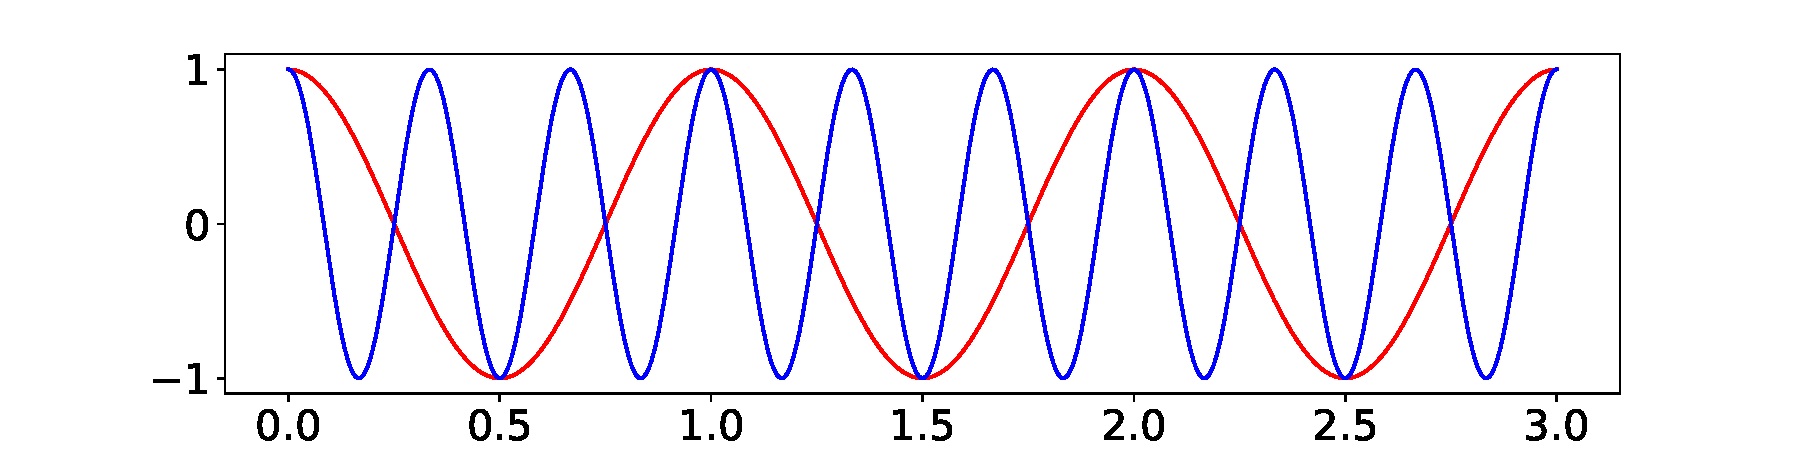
\includegraphics[width=0.7\textwidth]{../img/cosinus.pdf}
\end{figure}
The associated PSD functions .  
 
\centering
\begin{tikzpicture}[scale=0.6]
\makeatletter
\begin{axis}[axis lines=middle,xmin=-3.3,xmax=3.3,ymin=-0.5,ymax=1]
\addplot +[dirac, color = blue] coordinates {(-3,0.5) (3,0.5)};
\addplot +[dirac, color = red] coordinates {(-1,0.5) (1,0.5)};
\end{axis}

\draw [black,thick] (8,4) -- (12,5); 
\draw (12,5) node[right]{$\L_2=1/\sqrt{2}$};
\draw [black,thick] (8,2) -- (12,1);
\draw (12,1) node[right]{$W_2=2$};
\end{tikzpicture}
\end{frame}




\begin{frame}{\red{Definition:} The Wasserstein-Fourier distance}
\thispagestyle{empty}
\begin{definition}
For two signals $x$ and $y$ belonging to two different classes of time series, we denote by
\begin{itemize}
\item[$\bullet$] $[x]$ and $[y]$ their respective class
\item[$\bullet$] $s_x$ and $s_y$ their respective normalised PSD (NPSD)
\end{itemize}
We define the proposed \textit{Wasserstein-Fourier} (WF) distance:
$$\WF{x}{y}=W_2(s_x,s_y).$$
\end{definition}

\begin{theorem}
WF is a distance over the space of equivalence classes of time series
sharing the same NPSD.
\end{theorem}
\vfill

\noindent \footnotesize E. Cazelles, A. Robert \& \textbf{F. Tobar}, The Wasserstein-Fourier Distance for Stationary Time Series. \emph{IEEE Trans.~on Signal Processing} 2021.

\end{frame}

\begin{frame}{Basics properties of the WF distance}
    Time shifting : $x(t)=y(t-t_0)$.\\
    \begin{minipage}[c]{0.2\linewidth}
        \begin{figure}
            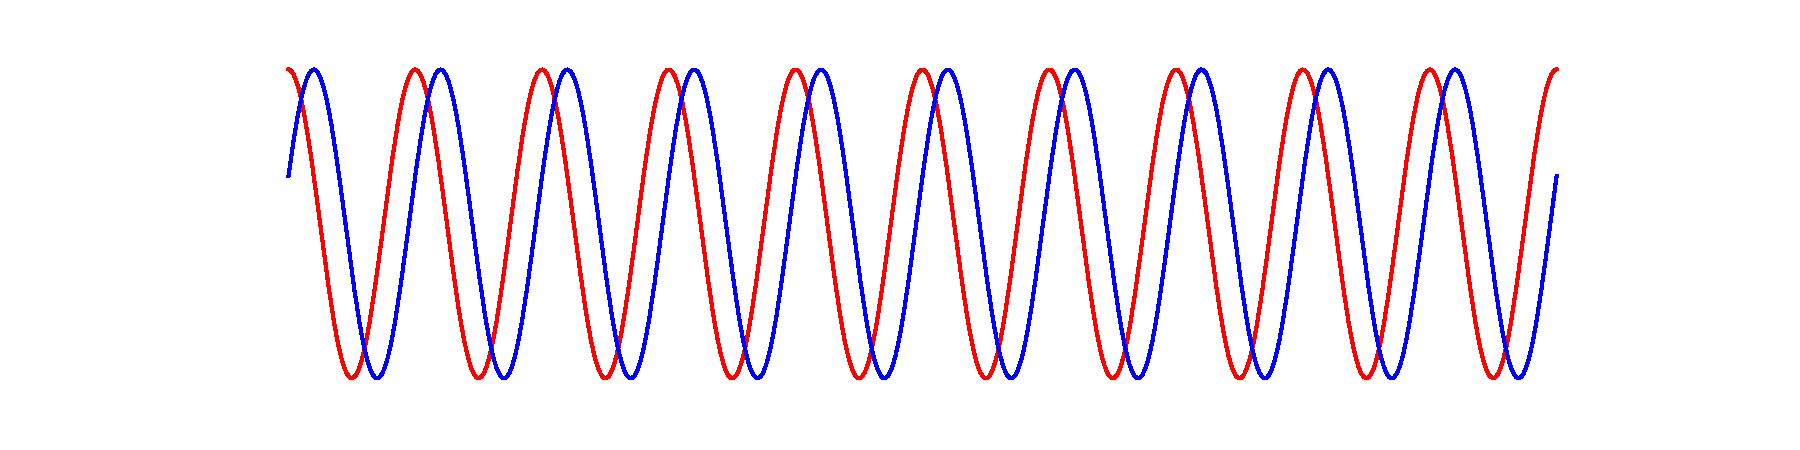
\includegraphics[scale=0.22]{../img/time_shift.pdf}
        \end{figure}
    \end{minipage}\hspace{4cm}
    \begin{minipage}[c]{0.4\linewidth}
        $$\WF{x}{y}=0$$
    \end{minipage}

    Time scaling : $x(t)=y(at), a>0$.\\
    \begin{minipage}[c]{0.2\linewidth}
        \begin{figure}
            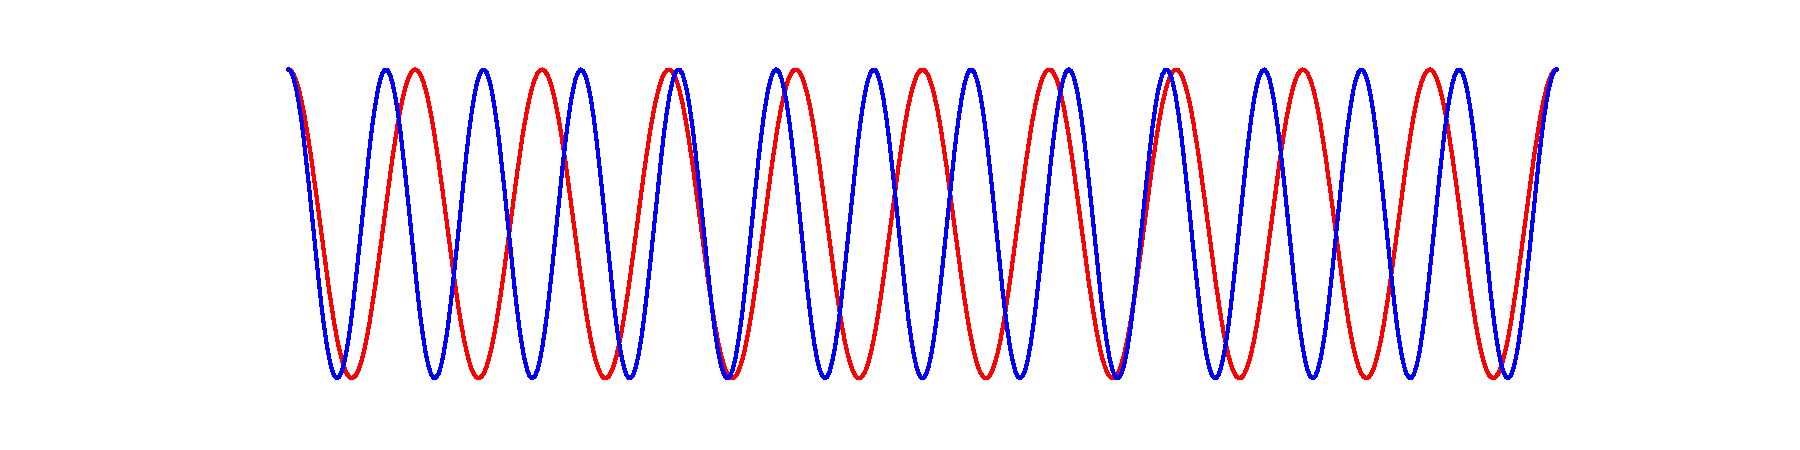
\includegraphics[scale=0.22]{../img/time_scaling.pdf}
        \end{figure}
    \end{minipage}\hspace{4cm}
    \begin{minipage}[c]{0.4\linewidth}
        $$\WF{x}{y}=\vert a-1\vert(\E{\vert Y\vert^2}_{s_y})^{\frac{1}{2}}$$
    \end{minipage}

    Frequency shifting : $x(t)=e^{2i\pi\xi_0t}y(t)$.\\
    \begin{minipage}[c]{0.2\linewidth} 
        \begin{figure}
            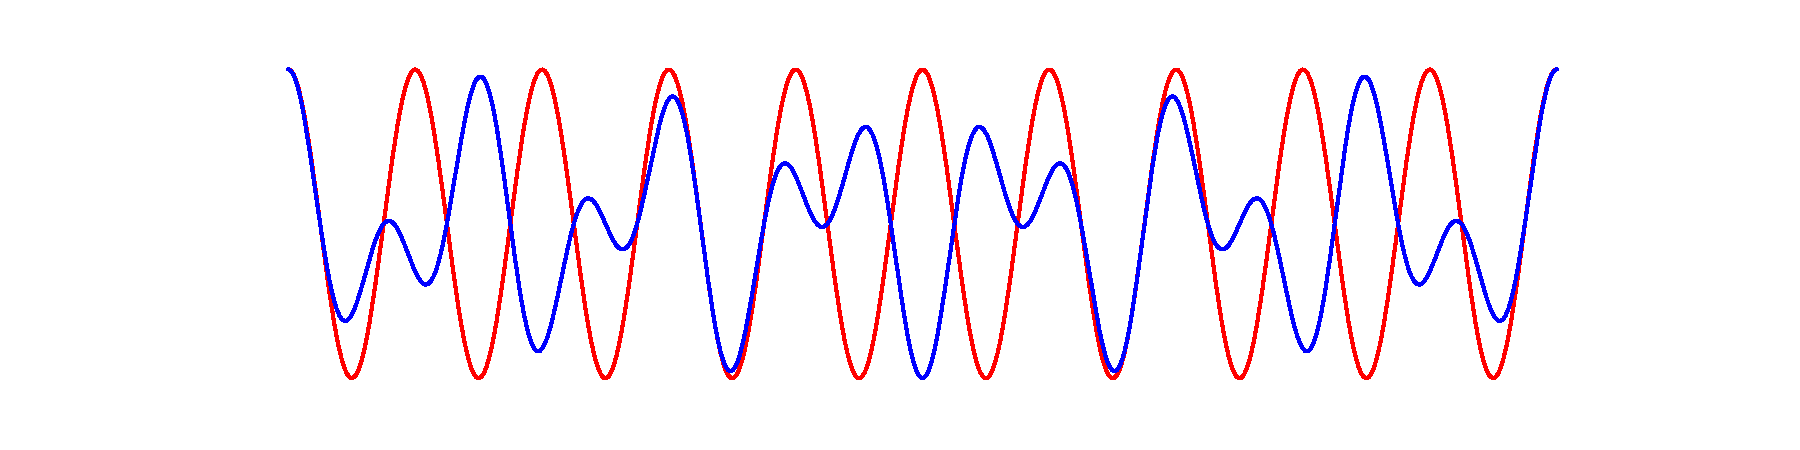
\includegraphics[scale=0.22]{../img/freq_shift.pdf}
        \end{figure}
    \end{minipage}\hspace{4cm} 
        \begin{minipage}[c]{0.4\linewidth}
            $$\WF{x}{y}=\vert \xi_0\vert$$
        \end{minipage}
\end{frame}


\begin{frame}{How to interpolate two time series?}
\textbf{The usual $\L_2$ path:} a superposition of two signals
$$x_{\gamma}(t)=\gamma \red{x_1(t)}+(1-\gamma)\blue{x_2(t)}, \quad \gamma\in [0,1],$$
\textbf{Example:} For EEG, the $\L_2$ average of multiple responses to a common stimulus would probably convey little information about the true average response and it is likely to quickly vanish due to the random phases.

\uncover<2->{   \textbf{Toy example: \uncover<8->{\red{The WF path i.e. Wasserstein interpolation in the frequency domain}}}

\begin{minipage}[c]{0.3\linewidth}
\begin{figure}
\begin{tikzpicture}
\draw [black] (0,2.5) node[above]{Time domain};
\only<2>{\draw (0,-0.3) node[above]{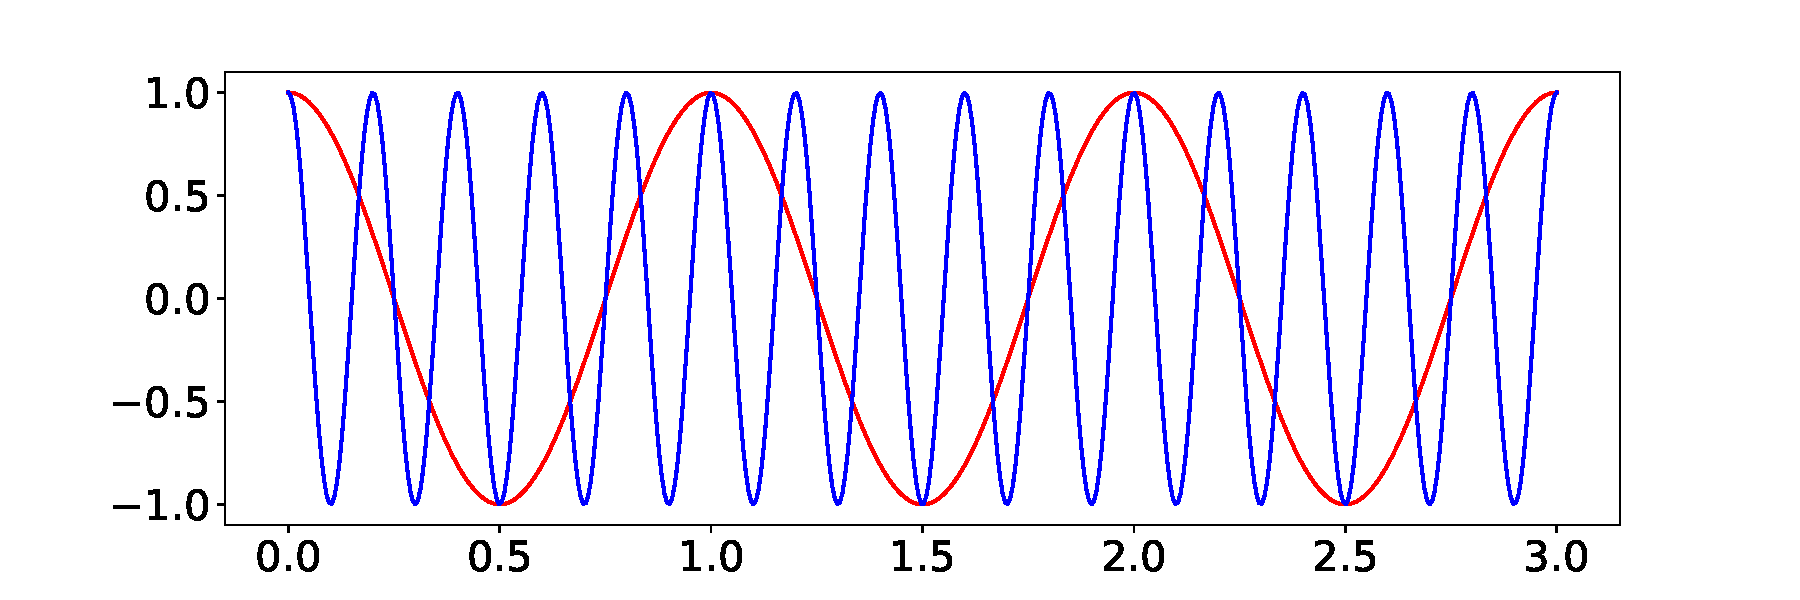
\includegraphics[scale=0.25]{../img/interp_both.pdf}};}
\only<3>{\draw (0,-0.3) node[above]{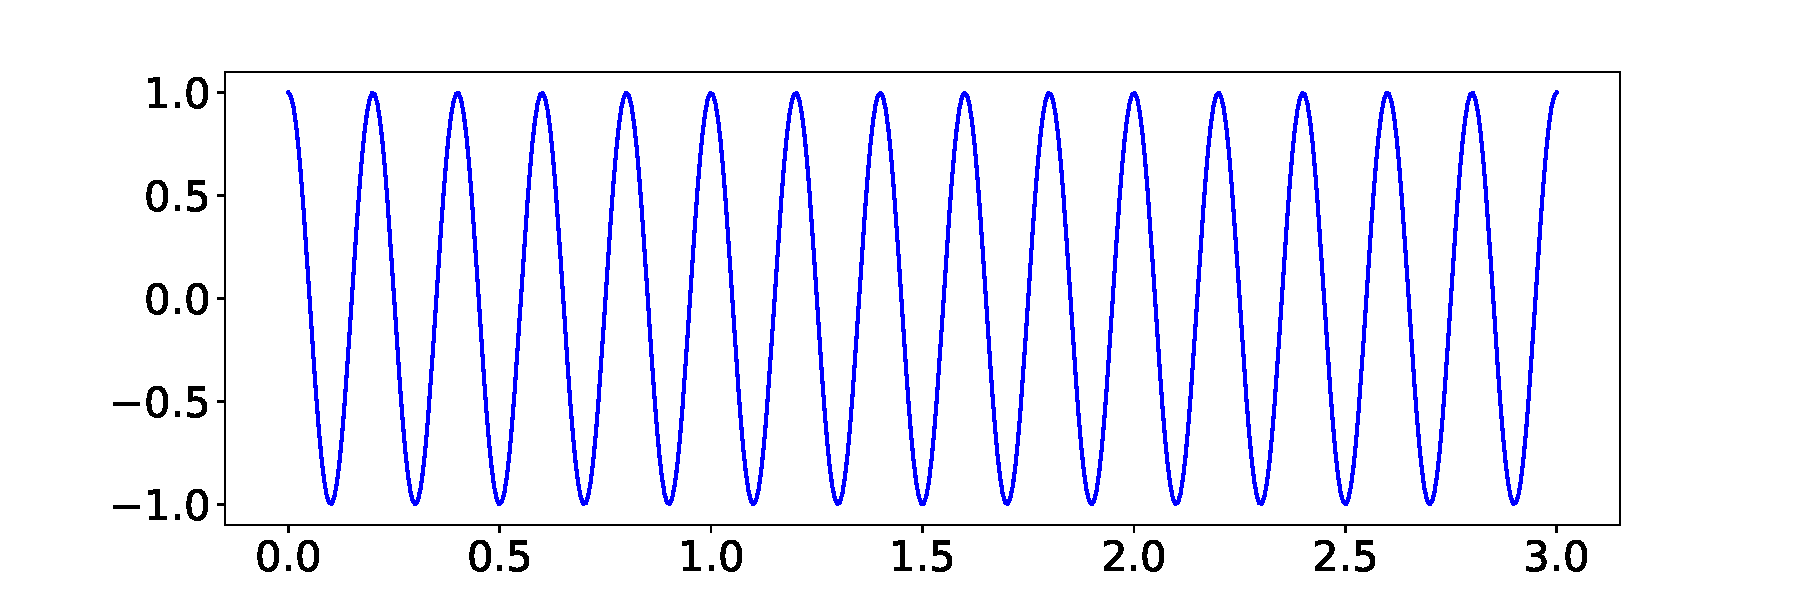
\includegraphics[scale=0.25]{../img/eucli0.pdf}};}
\only<4>{\draw (0,-0.3) node[above]{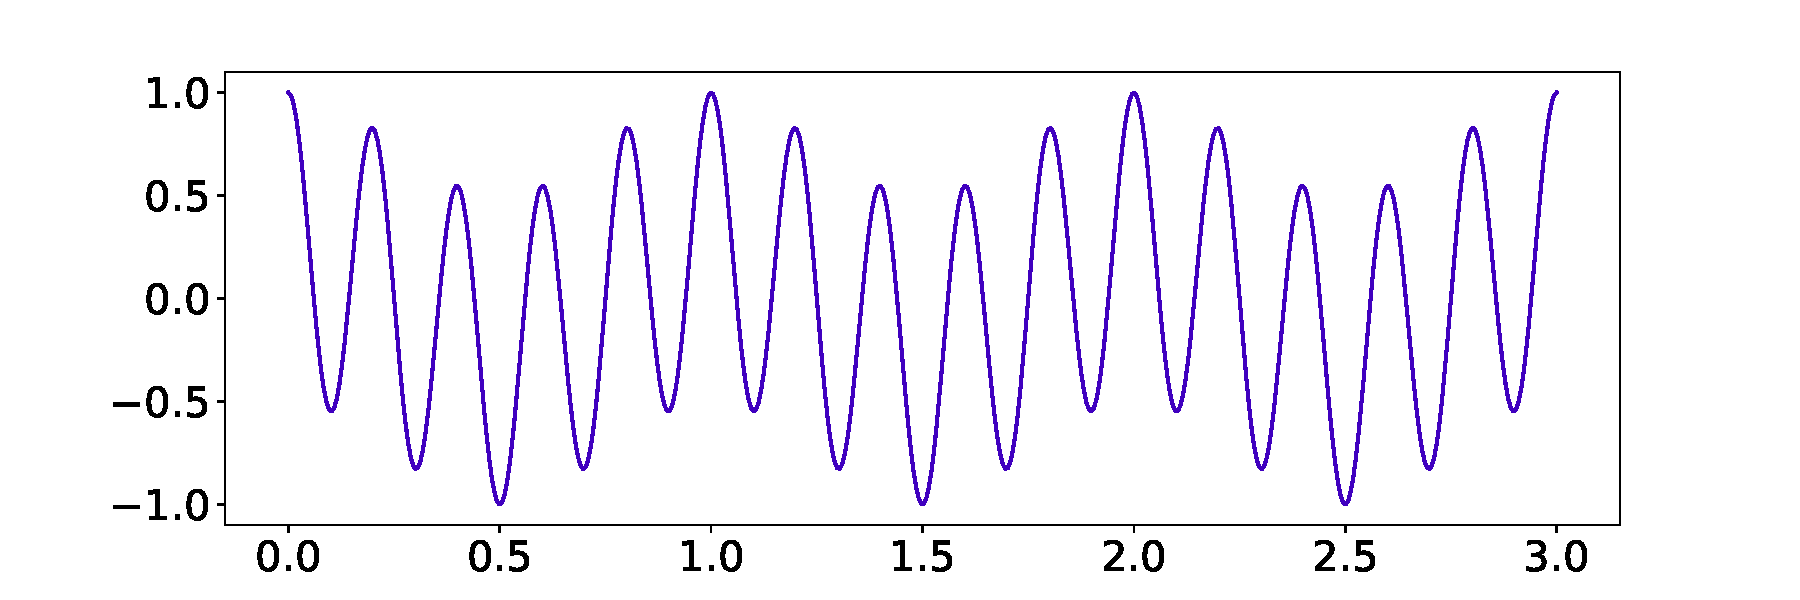
\includegraphics[scale=0.25]{../img/eucli1.pdf}};}
\only<5>{\draw (0,-0.3) node[above]{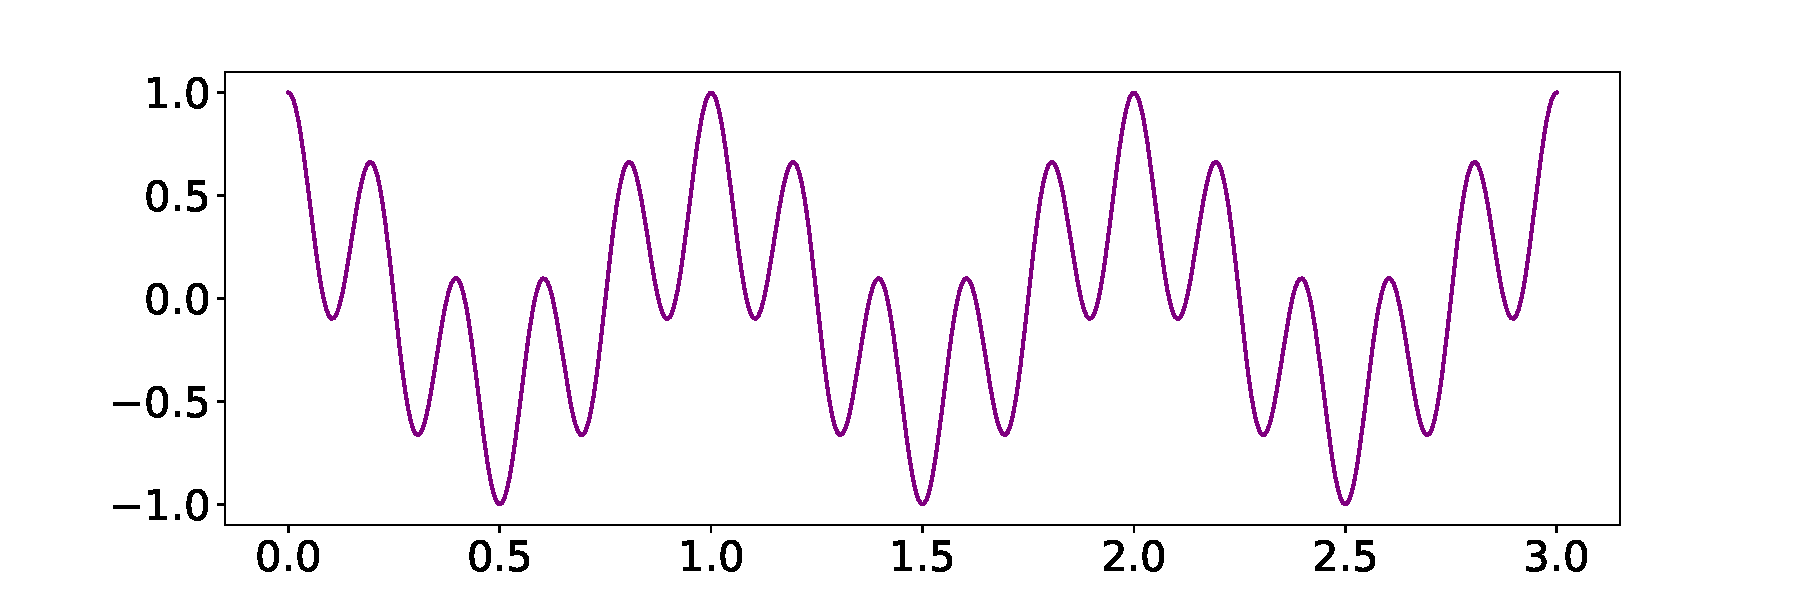
\includegraphics[scale=0.25]{../img/eucli2.pdf}};}
\only<6>{\draw (0,-0.3) node[above]{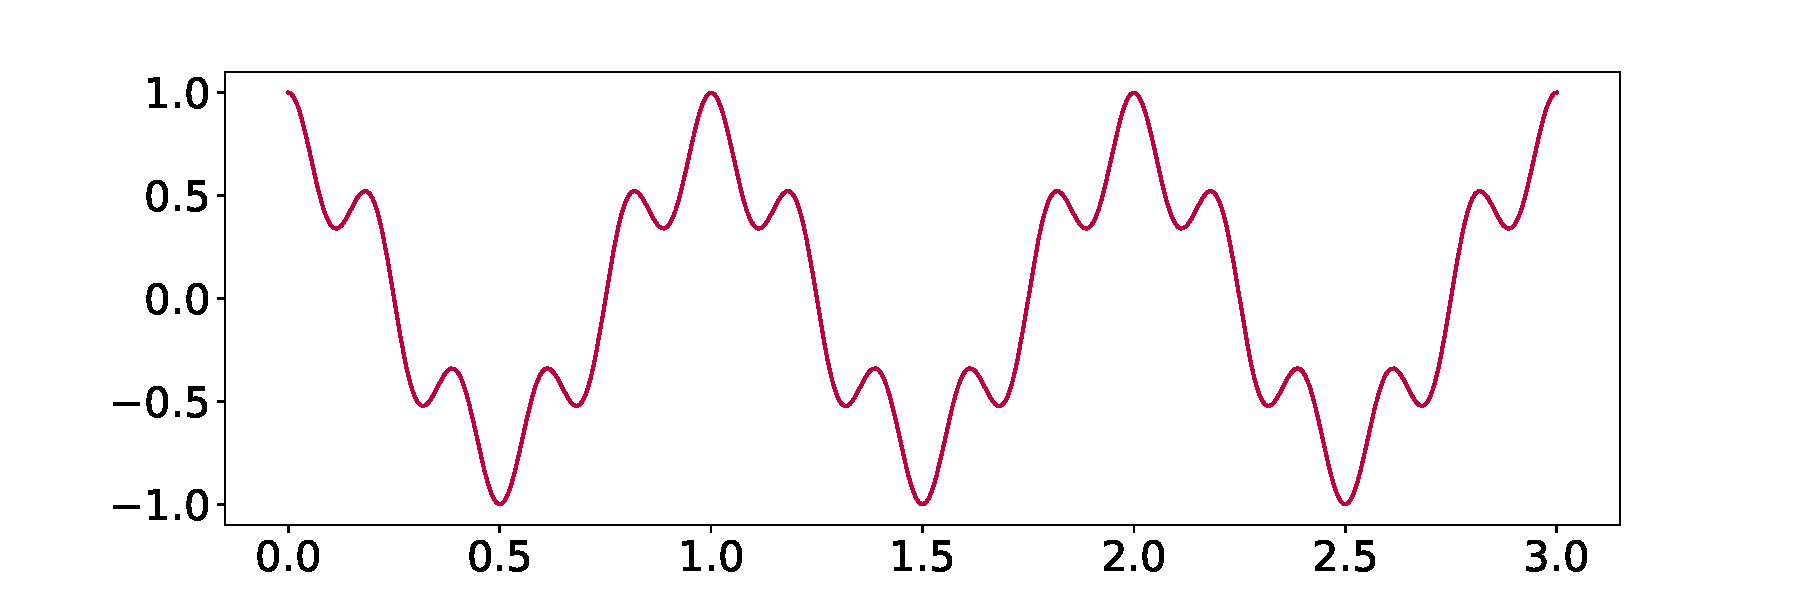
\includegraphics[scale=0.25]{../img/eucli3.pdf}};}
\only<7>{\draw (0,-0.3) node[above]{\includegraphics[scale=0.25]{../img/eucli4.pdf}};}
\only<8>{\draw (0,-0.3) node[above]{\includegraphics[scale=0.25]{../img/interp_both.pdf}};}
\only<9>{\draw (0,-0.3) node[above]{\includegraphics[scale=0.25]{../img/wass0.pdf}};}
\only<10>{\draw (0,-0.3) node[above]{\includegraphics[scale=0.25]{../img/wass1.pdf}};}
\only<11>{\draw (0,-0.3) node[above]{\includegraphics[scale=0.25]{../img/wass2.pdf}};}
\only<12>{\draw (0,-0.3) node[above]{\includegraphics[scale=0.25]{../img/wass3.pdf}};}
\only<13>{\draw (0,-0.3) node[above]{\includegraphics[scale=0.25]{../img/wass4.pdf}};}
\end{tikzpicture}
\end{figure}
\end{minipage}\hspace{3.5cm}
\begin{minipage}[c]{0.3\linewidth}
\begin{tikzpicture}[scale=0.5]
\only<3>{\draw [blue] (0,4.4) node[above]{$\gamma=0$};}
\only<4>{\draw [color1] (0,4.4) node[above]{$\gamma=0.25$};}
\only<5>{\draw [color2] (0,4.4) node[above]{$\gamma=0.5$};}
\only<6>{\draw [color3] (0,4.4) node[above]{$\gamma=0.75$};}
\only<7>{\draw [red] (0,4.4) node[above]{$\gamma=1$};}
\only<9>{\draw [blue] (0,4.4) node[above]{$\gamma=0$};}
\only<10>{\draw [color1] (0,4.4) node[above]{$\gamma=0.25$};}
\only<11>{\draw [color2] (0,4.4) node[above]{$\gamma=0.5$};}
\only<12>{\draw [color3] (0,4.4) node[above]{$\gamma=0.75$};}
\only<13>{\draw [red] (0,4.4) node[above]{$\gamma=1$};}
\uncover<8->{\draw [black] (3,6) node[above]{Frequency domain};
\makeatletter
\begin{axis}[axis lines=middle,xmin=-5.3,xmax=5.3,ymin=-0.2,ymax=1]
\only<8>{\addplot +[dirac, color = blue] coordinates {(-5,0.5) (5,0.5)};
\addplot +[dirac, color = red] coordinates {(-1,0.5) (1,0.5)};}
\only<9>{\addplot +[dirac, color = blue] coordinates {(-5,0.5) (5,0.5)};}
\only<10>{\addplot +[dirac, color = color1] coordinates {(-4,0.5) (4,0.5)};}
\only<11>{\addplot +[dirac, color = color2] coordinates {(-3,0.5) (3,0.5)};}
\only<12>{\addplot +[dirac, color = color3] coordinates {(-2,0.5) (2,0.5)};}
\only<13>{\addplot +[dirac, color = red] coordinates {(-1,0.5) (1,0.5)};}
\end{axis}}
\end{tikzpicture}
\end{minipage}
}
\end{frame}

\begin{frame}{An interpolation path between two times series}
\begin{tikzpicture}
\draw [blue] (0.8,0) node[above]{Time domain};
\draw [blue] (7.5,0) node[above]{Frequency domain};
\draw [blue, dashed, line width=0.8pt] (2.8,0.5) -- (2.8,0);
\draw [blue, dashed, line width=0.8pt] (2.8,-0.9) -- (2.8,-2.9);
\draw [blue, dashed, line width=0.8pt] (2.8,-3.8) -- (2.8,-6.8); 

\draw [purple] (0.8,-1.5) node[above]{\CVI{$x_1,x_2$}};
\draw (1,-5.5) node[above]{\begin{minipage}[c]{0.28 \linewidth}
\CM{$(x_{\gamma})_{\gamma\in[0,1]}$}

Interpolant between\\ \CVI{$x_1$} and \CVI{$x_2$}
\end{minipage}};

\draw [black] (2.9,-0.6) node[above]{NPSD};
\draw [->] [black, thick,rounded corners=10pt] (1.2,-1) to[bend left=25] (4.5,-1.1);
\draw [->] [black, thick,rounded corners=10pt] (5.5,-1.6) to[bend left=20] (6.8,-4.2);

\draw [black] (3.2,-3.5) node[above]{Inverse Fourier transform};
\draw [->] [black, thick,rounded corners=10pt] (6,-4.2) to[bend right=20] (1.2,-4);


\draw [blue] (5,-1.7) node[above]{\red{$s_1, s_2$}};
\draw (9,-0.5) node[below]{\begin{minipage}[c]{0.4 \linewidth}
McCann's interpolant (or constant-speed geodesic, Ambrosio et. al (2008)) \CO{$(g_{\gamma})_{\gamma\in [0,1]}$} between \red{$s_1$} and \red{$s_2$}.
\end{minipage}};    

\draw (8.8,-4) node[below]{\begin{minipage}[c]{0.7 \linewidth}
$$\CO{g_{\gamma} = p_{\gamma}\#\pi^{\ast}}, \gamma\in[0,1]$$
\begin{itemize}
\item[$\bullet$] $p_{\gamma}(u,v) = (1-\gamma)u+\gamma v$, for $u, v\in\R$
\item[$\bullet$] $\pi^{\ast}$ optimal transport plan between \red{$s_1$} and \red{$s_2$}
\item[$\bullet$] $\# =$ pushforward operator
\end{itemize}
\end{minipage}};
\end{tikzpicture}
\end{frame}



\begin{frame}{Example: interpolation for the \emph{C. Elegans} database}
\begin{figure}
\centering
\includegraphics[width=0.475\textwidth]{../img/worms_geodesic_sameclass.pdf}
\includegraphics[width=0.475\textwidth]{../img/worms_euclidean_sameclass.pdf}
  {10-step interpolation $(x_{\gamma})_{\gamma\in [0,1]}$ between two signals from the {\em C.~elegans} database using the proposed WF distance (top) and the Euclidean distance (bottom): the true signals are shown in solid blue and red, while the interpolations are colour-coded with respect to $\gamma$.}
\end{figure}
\end{frame}




\begin{frame}{Logistic regression of time series}
For two classes $C_0$ and $C_1$, one defines a binary classification of a sample $s$ as
$$p(C_0\vert s)=\frac{1}{1+e^{-\red{\alpha}+\red{\beta} d(s,\bar{s_0})+\red{\gamma} d(s,\bar{s_1})}},$$
where $d$ is a divergence $(\L_2, KL, W_2)$ and $\bar{s_i}$ sums up the information of class $C_i$.

\begin{itemize}
\item[$\bullet$] $\L_2$ and $KL$ cases:
$$\bar{s}\in \underset{s}{\argmin}\frac{1}{n}\sum_{i=1}^n\Vert s_i-s\Vert^2=\frac{1}{n}\sum_{i=1}^n s_i.$$
\item[$\bullet$] $W_2$ case: a \textbf{Wasserstein barycentre} of a family $(s_i)_{i=1,\ldots,n}$ of distributions is given by
$$\bar{s}\in \underset{s}{\argmin}\frac{1}{n}\sum_{i=1}^nW_2^2(s_i,s).$$
\end{itemize}
\end{frame}

\begin{frame}{Logistic regression of time series}
\begin{figure}
\includegraphics[trim={0 180 0 180},clip,width=1\textwidth]{../img/toy_example2.pdf}
{Illustration of the linear separability made possible by the Wasserstein-Fourier distance.}
\end{figure}
\end{frame} 

\begin{frame}{Real-world example: urban audio recordings\footnote{Urbansound8k dataset}}
\begin{table}[h!]
\centering
\small
\begin{tabular}{p{2.5cm}p{2.5cm}p{2.5cm}p{2.5cm}} \toprule

                    & $\mathcal{L}_{W_2}$          & $\mathcal{L}_{\L_2}$ & $\mathcal{L}_{KL}$         \\ \midrule 
air conditioner     & \textbf{0.732} ($\pm0.072$)  & 0.718 ($\pm0.047$) & 0.650 ($\pm0.090$)           \\
car horn            & 0.588 ($\pm0.077$)           & 0.743 ($\pm0.043$) & \textbf{0.790} ($\pm0.037$)  \\
children playing    & \textbf{0.751} ($\pm0.027$)  & 0.685 ($\pm0.031$) & 0.736 ($\pm0.023$)           \\ \midrule
dog bark            & \textbf{0.743} ($\pm0.040$)  & 0.720 ($\pm0.033$) & 0.728 ($\pm0.040$)           \\ 
drilling            & \textbf{0.827} ($\pm0.027$)  & 0.826 ($\pm0.026$) & 0.817 ($\pm0.026$)           \\ 
engine idling       & 0.767 ($\pm0.041$)           & 0.733 ($\pm0.051$) & \textbf{0.791} ($\pm0.042$)  \\ \midrule
jackhammer          & 0.645 ($\pm0.087$)           & 0.585 ($\pm0.095$) & \textbf{0.669} ($\pm0.059$)  \\
siren               & 0.803 ($\pm0.062$)           & 0.878 ($\pm0.034$) & \textbf{0.897} ($\pm0.034$)  \\
street music        & 0.792 ($\pm0.030$)           & 0.782 ($\pm0.025$) & \textbf{0.812} ($\pm0.029$)  \\ \bottomrule
\end{tabular}
\vspace{1em}
\caption{Classification results for the class \textit{gun shot} against the 9 remaining classes.}
\end{table}
\end{frame}


\begin{frame}{Geodesic path for Gaussian processes}
Gaussian process $\leftrightarrow$ Kernel $\leftrightarrow$ PSD.
\begin{figure}
\includegraphics[trim={0 150 0 150},clip,width=1\textwidth]{../img/sinc_gaus_sin2.pdf}
\end{figure}
\centering
\bred{Spoiler:} GPs can be trained in this way at a linear cost
\end{frame}

\begin{frame}[plain]{How Gaussian processes are trained}
    \noindent\bred{Maximum likelihood}: Standard (very expensive) approach.\vspace{2em}


    \noindent\bred{Covariance-based metrics}: Compute sample covariance and apply, e.g., $L_p$ distances.


    \begin{figure} 
            \centering
            %\includegraphics[width=0.8\textwidth]{figs/temporal_metric_diag.pdf}
        \end{figure}

     \noindent\bred{Frequency-based metrics}: Compute \textbf{Periodogram} and use any density-based metric: KL, Bergamn, Itakura-Saito, and Wasserstein. 
    
        \begin{figure} 
            \centering
            \includegraphics[width=0.9\textwidth]{../img/spectral_metric_diag.pdf}
        \end{figure}


\end{frame}


\begin{frame}[plain]{An interesting case}
    Let us consider: 
        \begin{itemize}
        \item Metric: The \textit{Wasserstein} distance applied to the PSD, i.e., $W_2$ on $S=\fourier{K}$.
        \item A Location-scatter family of PSD: $  \left\{S_{\mu,\sigma}(\xi) = \frac{1}{\sigma} S_{0,1} \left(\frac{\xi-\mu}{\sigma}\right), \mu\in\R,\sigma\in\R_+\right\}$ 
    \end{itemize}
    \begin{theorem} 
\label{thm:convexWF}
For a  location-scale family with prototype $S_{0,1}$, the minimiser of $W_2(S, S_{\mu,\sigma})$ is unique, given by 
\begin{equation}
  \mu^* = \int_0^1 Q(p)d p \qquad \mbox{and} \qquad
  \sigma^* = \frac{1}{\int_0^1 Q_{0,1}^2(p)d p}\int_0^1 Q(p) Q_{0,1}(p)d p \label{eq:soln_mu_sigma}
\end{equation}
where $Q$ is the quantile function of $S$. The PSD $S$ does not need to be location-scale.
\end{theorem}
\bred{Corollary:} Training a GP with the Wasserstein distance has a cost $\mathcal{O}(n)$. I.e., no need of a gradient flow, as solution is exact and closed form.
\end{frame}




\begin{frame}[plain]{Theoretical aspects}
    \bred{Does it converge?} I.e., is it true that
    \begin{equation}
        \theta_n^\star = \argmin D(\hat S_n, S_\theta) \xrightarrow[n \to \infty]{a.s.} \theta^\star = \argmin D(S, S_\theta)
    \end{equation}
    yes it is, provided that: 
    \vspace{1em}
    \begin{itemize}
        \item \textbf{Metric.} $D$ is either the Wasserstein-$p$ or the $L_p$ distances with $p\in\{1,2\}$
        \item \textbf{Estimator of PSD.} $D(\hat S_{n}, S)\xrightarrow [n\to \infty]{a.s.} 0$
        \item \textbf{Identifiability.} $\theta_n\xrightarrow[n\to \infty]{} \theta \iff D(S_{\theta_n}, S_\theta)\to 0$; 
        \item \textbf{Compactness.} the parameter space  $\Theta$ is compact.
    \end{itemize}

    \vspace{2em}
    \flushright ** This applies to temporal (covariance) distances too


\end{frame}




\begin{frame}[plain]{OT-powered GP training: Linear complexity }

\begin{itemize}
    \item Computation time vs number of observations
    \item Exact case ($W_2$ distance and location-scale family)
    \item \textbf{Unevenly-sampled} observations from an single component SM kernel ($\mu=0.05, \sigma=0.01$) in the range $[0,1000]$
    \item Compared against: ML estimate starting from the OT value (full GP, 100 iterations), and sparse GP using 200 pseudo inputs
\end{itemize}

\begin{figure}[ht]
\centering
  \includegraphics[width=0.7\textwidth]{../img/exp2.pdf}
  \label{fig:comp_cost}
\end{figure} 
    
\end{frame}






%\section{Closing remarks}

\begin{frame}{What we did not see}
\begin{itemize}
    \item Dual formulation of the Kantorovich problem
    \item Computational OT
    \item Multimarginal OT
    \item Unbalanced OT
    \item Partial OT
    \item Weak OT
    \item Particular cases with closed form
\end{itemize}
\end{frame}


\begin{frame}{Conclusions \& the future}
    \begin{itemize}
        \itemsep1em  
        \item OT is now in the toolkit for many fields spanning \bblue{data analysis}, \bblue{machine learning}, data science and AI.
        \item OT defines a meaningful distance between distributions, and gives a procedure for \bblue{moving particles to minimise such distance}
        \item Some open challenges: 
        \begin{itemize}
            \item computational \bblue{complexity}
            \item \bblue{curse of dimensionality:} samples for approximations grow exponentially with the dimension
            \item \bblue{robustness of the solution} with statistical guarantees (noise? outliers?)
            \item OT on \bblue{different spaces} than Euclidean ones
            \item adding some extra constraints (such as temporal consistency)
        \end{itemize}
        \end{itemize}
\end{frame}











\begin{frame}[plain]
    \titlepage
\end{frame}



\appendix



\begin{frame}
    \Large \bblue{Appendix: what we didn't see}
\end{frame}







\begin{frame}{Dual formulation}

Recall the primal formulation: $\OT({\mu},{\nu}) = \inf _{\pi\in\Pi(\mu,\nu)} \iint c(x,y)\d\pi(x,y)$
\begin{block}{}
\bblue{Dual problem}
$$\OT({\mu},{\nu}) = \sup_{(\phi,\psi)\in\Phi_c} \left(\int_{\XX} \phi d{\mu} + \int_{\XX} \psi d{\nu}\right),$$
where
$$\Phi_c : = \left\{(\phi,\psi)\in L_1(\mu)\times L_1(\nu),\ \mbox{s.t.}\ \phi(x) + \psi(y)\leq c(x,y)\right\}.$$
\end{block}

{\vspace{0.3cm}\begin{itemize}
\item[$\bullet$] $\phi$ and $\psi$ are scalar function also known as \bblue{Kantorovich potentials}
\item[$\bullet$] Primal-dual relationship: the support of $\pi\in\Pi^{\ast}(\mu,\nu)$ is such that $\phi(x)+\psi(y) = c(x,y)$.
\end{itemize}}

{\vspace{0.3cm} In the discrete setting:
$$\int_{\XX} \phi d\left({\sum_{i=1}^n\mu_i\delta_{x_i}}\right) + \int_{\XX} \psi d\left({\sum_{j=1}^m\nu_j\delta_{y_i}}\right) = \sum_{i=1}^n\mu_i\underbrace{\phi(x_i)}_{\alpha_i} + \sum_{j=1}^m\nu_j\underbrace{\psi(y_j)}_{\beta_j}$$
and $\Phi_c$ becomes $\{(\alpha,\beta)\in\R^n\times\R^m \ \mbox{s.t.}\ \alpha_i+\beta_j\leq c(x_i,y_j)\}$
}

\end{frame}



\begin{frame}{Interpretation of Kantorovich duality (discrete)}
$$\OT({\mu},{\nu}) = \underset{\pi\in\Pi(\mu,\nu)}{\min} \langle C, \pi \rangle = \max_{(\alpha,\beta)\in D_c} \ \langle \alpha,{\mu}\rangle + \langle \beta, {\nu}\rangle$$
with
$$D_c := \{(\alpha,\beta)\in\R^n\times\R^m \ \mbox{such that}\ \forall (i,j)\in\{1,\ldots,n\}\times\{1,\ldots,m\}, \alpha_i+\beta_j\leq C_{ij}\}$$

\begin{center}
\includegraphics[width=0.9\textwidth]{../img/wine_load1.pdf}
\end{center}

\end{frame}


\begin{frame}{Intuition: the shipper's problem}
One vendor sets the following:
\begin{itemize}
\item[$\bullet$] $\alpha_i$ = price for \textbf{loading} a kilo of grapes at place $\er{x_i}$ (no matter which plan it goes)
\item[$\bullet$] $\beta_j$ = price for \textbf{unloading} a kilo of grapes at place $\eb{y_j}$ (no matter from which vineyard it came from)
\end{itemize}

\begin{center}
\includegraphics[width=0.9\textwidth]{../img/wine_load2.pdf}
\end{center}

\end{frame}

\begin{frame}{Intuition: the shipper's problem}

\begin{itemize}
\item[$\bullet$] There are exactly $\er{\mu_i}$ units at vineyard $\er{x_i}$ and $\eb{\nu_j}$ needed at plant $\eb{y_j}$; the vendor asks the price \bblue{(that she wants to maximize!)}
$$\langle\alpha, \er{\mu}\rangle + \langle\beta, \eb{\nu}\rangle$$
\visible<1-2>{\item[$\bullet$] Negative price are allowed!}
\visible<1-2>{\item[$\bullet$] Does the vendor have a competitive offer? Her pricing scheme implies that transferring one kilo of grapes from vineyard $\er{x_i}$ to plant $\eb{y_j}$ costs exactly $\alpha_i+\beta_j$.}
\visible<2>{\item[$\bullet$] \blue{Recall the primal problem:} the cost of shipping one unit from ${x_i}$ to ${y_j}$ is $C_{i,j}$.}
\visible<2>{\item[$\bullet$] Feasible deal for the vendor requires that  $\alpha_i+\beta_j\leq C_{ij}$.}
\visible<2>{\item[$\bullet$] The winery checks that the vendor proposition is a better deal by
\begin{align*}
\sum_{i,j} \pi_{ij}C_{ij}\geq \sum_{i,j} \pi_{ij}(\alpha_j+\beta_j) &= \left(\sum_i\alpha_i\sum_j\pi_{ij}\right) + \left(\sum_j\beta_j\sum_i\pi_{ij}\right)= \langle\alpha, \mu\rangle + \langle\beta, \nu\rangle
\end{align*}}.
\end{itemize}
\visible<2>{
    \bblue{Critically, when $c(x,y) = |x-y|$,  $\alpha = -\beta$, therefore $\OT(\mu,\nu) = \max_\alpha \langle\alpha, \mu\rangle - \langle\alpha, \nu\rangle$}
}


\end{frame}





\begin{frame}{\bred{Example 5:} Wasserstein GANs}


\begin{textblock}{0.45}(0.65,0.12)
\bblue{\large Recall (standard) GANs}
\end{textblock}
\vspace{-2em}
    \begin{figure}
        \centering
            \includegraphics[width=0.7\textwidth]{../img/gan_diag.pdf}
        \end{figure}
\bred{Notice the remarkable similarity between the objectives of the (dual) OT formulation and GANs}
\end{frame}

\begin{frame}{\bred{Example 5:} Wasserstein GANs}
\framesubtitle{GANs vs WGANs: Implementation details}

\begin{minipage}{0.32\textwidth}
    \begin{itemize}
        \item Discriminator loss no longer a likelihood fn 
        \item Optimised with RMSProp
        \item Loss for $D$ and $G$ have the same form (Kantorovich potential, $p=1$)
        \item Discriminator's inner loop training $n_\text{critic}$ no longer equal to 1
        \item Learned parameters are clipped to ensure $||f||_L=1$
    \end{itemize}
\end{minipage}
\begin{minipage}{0.32\textwidth}
        \begin{figure}
        \centering
            \includegraphics[width=0.95\textwidth]{../img/gan_mnist.pdf}
            \centerline{\bblue{GAN}}
        \end{figure}
\end{minipage}
\begin{minipage}{0.32\textwidth}
            \begin{figure}
        \centering
            \includegraphics[width=0.95\textwidth]{../img/wgan_mnist.pdf}
            \centerline{\bred{W}\bblue{GAN}}
        \end{figure}
\end{minipage}
\begin{textblock}{0.45}(0.45,0.5)
    \bred{
    \underline{
        Notebooks: \href{https://github.com/felipe-tobar/OT-tutorial-MLSP-2024/blob/main/Codes/gan.ipynb}{gan.ipynb} \& \href{https://github.com/felipe-tobar/OT-tutorial-MLSP-2024/blob/main/Codes/wgan.ipynb}{wgan.ipynb} 
    }}\end{textblock}

\end{frame}



\end{document}